% !TEX encoding = UTF-8 Unicode
\documentclass[10pt, aspectratio=149]{beamer}

% Beamer Packages
\usetheme{metropolis}
\usepackage{appendixnumberbeamer}
\graphicspath{{figs/}}
\usepackage{array, booktabs}
\usepackage{subfigure}
%\usepackage[scale=2]{ccicons}
%\usepackage{pgfplots}
%\usepgfplotslibrary{dateplot}

% Math
\usepackage{amsmath}
\usepackage{amsthm}
\usepackage{amssymb}
\usepackage{amsfonts}
\usepackage{latexsym}
\usepackage{algorithm}
\usepackage{algpseudocode}
\usepackage{eucal}
\usepackage{bm}

\usefonttheme[onlymath]{serif}

% Calligraphic Fonts 
\newcommand{\ca}{{\cal A}}
\newcommand{\cb}{{\cal B}}
\newcommand{\cc}{{\cal C}}
\newcommand{\cd}{{\cal D}}
\newcommand{\ce}{{\cal E}}
\newcommand{\cf}{{\cal F}}
\newcommand{\ch}{{\cal H}}
\newcommand{\cl}{{\cal L}}
\newcommand{\cm}{{\cal M}}
\newcommand{\co}{{\cal O}}
\newcommand{\cp}{{\cal P}}
\newcommand{\ct}{{\cal T}}
\newcommand{\cz}{{\cal Z}}

% Bold Fonts
\newcommand{\one}{{\mathbf{1}^{\prime}}}
\newcommand{\bu}{{\mathbf u}}
\newcommand{\bx}{{\mathbf x}}
\newcommand{\bX}{{\mathbf X}}
\newcommand{\bn}{{\mathbf N}}
\newcommand{\bo}{{\mathbf O}}
\newcommand{\bp}{{\mathbf P}}
\newcommand{\br}{{\mathbf R}}
\newcommand{\bs}{{\mathbf s}}
\newcommand{\bS}{{\mathbf S}}
\newcommand{\bz}{{\mathbf Z}}
\newcommand{\balpha}{{\boldsymbol\alpha}}
\newcommand{\bbeta}{{\boldsymbol\beta}}
\newcommand{\bdelta}{{\boldsymbol\delta}}
\newcommand{\bpi}{{\boldsymbol\pi}}
\newcommand{\bmu}{{\boldsymbol\mu}}
\newcommand{\bsigma}{{\boldsymbol\sigma}}
\newcommand{\btheta}{{\boldsymbol\theta}}
\newcommand{\bGamma}{{\boldsymbol\Gamma}}

% Hollow Fonts
\newcommand{\expe}{{\mathbb E}}
\newcommand{\hn}{{\mathbb N}}
\newcommand{\bbt}{{\mathbb T}}
\newcommand{\hs}{{\mathbb S}}

% Arrows
\newcommand{\ra}{\rightarrow}
\newcommand{\la}{\leftarrow}
\newcommand{\lra}{\leftrightarrow}
\newcommand{\Ra}{\Rightarrow}
\newcommand{\La}{\Leftarrow}
\newcommand{\LRa}{\Longrightarrow}
\newcommand{\LLa}{\Longleftarrow}

% Operators
\DeclareMathOperator*{\argmax}{argmax}
\newcommand{\ov}{\overline}
\providecommand{\abs}[1]{\lvert#1\rvert}
\providecommand{\norm}[1]{\lVert#1\rVert}
\providecommand{\prob}[1]{\mathbb{P}(#1)}

%%%%%%%%%%%%%%%%%%%%%%%%%%

\title{Prediction of stock return series with \\ hidden Markov models}
%\subtitle{A modern beamer theme}
\date{June 9, 2016}
\author{\normalsize{Tian Gao}}
\institute{
    Supervised by Associate Professor Jianzhong Lin \\
    School of Mathematical Sciences \\
    Shanghai Jiao Tong University}
\titlegraphic{\vspace{3.7cm}\hspace{8.5cm}
\includegraphics[height=2.8cm]{sjtubadge.pdf}}
%\logo{\vspace{-0.97cm}
\includegraphics[height=0.5cm]{sjtubanner.pdf}}

%%%%%%%%%%%%%%%%%%%%%%%%%%

\begin{document}

\maketitle

%%%%%%%%%%%%%%%%%%%%%%%%%%

\begin{frame}{Table of Contents}
	\setbeamertemplate{section in toc}[sections numbered]
	\tableofcontents[hideallsubsections]
\end{frame}

%%%%%%%%%%%%%%%%%%%%%%%%%%

% !TEX encoding = UTF-8 Unicode

\section{\large Introduction}

%%%%%%%%%%%%%%%%%%%%

\subsection{Background}

\begin{frame}[fragile,t]{Background}
	\begin{center}
	\begin{tabular}{m{0.4\textwidth} m{0.4\textwidth}}
	\center
\includegraphics[width=0.3\textwidth]{renaissance.jpg} & 
	\center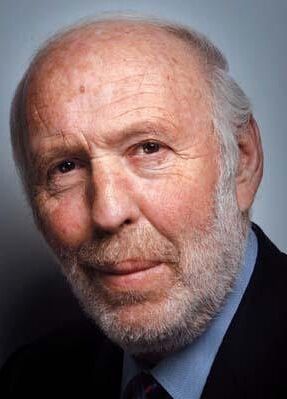
\includegraphics[width=1.5cm]{simmons.jpg}
	\end{tabular}
	\end{center}

	\begin{itemize}
	\item Quantitative finance analysis develops in China.
	\item Simple time series analysis techniques are incapable of capturing the market states.
	\item Dr.\,James H.~Simons implemented hidden Markov models (HMM)
		at Medallion Fund of Renaissance Technologies LLC.
	\end{itemize}

\end{frame}

%%%%%%%%%%%%%%%%%%%%

\subsection{Major Contributions and Key Spotlights}

\begin{frame}[fragile,t]{Major Contributions and Key Spotlights}
	% \begin{block}{Aim 1. System construction}
	% 	Construct the entire system for stock return series prediction, 
	% 	including data pre-processing, model construction and estimation, 
	% 	and eventually predictions with detailed analysis.
	% \end{block}

	% \begin{block}{Aim 2. Model estimation}
	% 	Estimate the HMM parameters in order to calibrate the model with accessible market data.
	% \end{block}

	% \begin{block}{Aim 3. Positive analysis}
	% 	Carry out empirical analysis on both Chinese and U.S. stock markets. 
	% 	Verify the effectiveness of the prediction system and provide detailed analysis and comparisons.
	% \end{block}

	% \begin{itemize}
	% 	\item \textbf{Aim 1. System construction} \\
	% 	Construct the entire system for stock return series prediction. \\
	% 	The system should include data pre-processing, model construction and estimation, 
	% 	and eventually predictions with detailed analysis.
	% 	\item \textbf{Aim 2. Model estimation} \\
	% 	Estimate the HMM parameters in order to calibrate the model with accessible market data.
	% 	\item \textbf{Aim 3. Positive analysis} \\
	% 	Carry out empirical analysis on both Chinese and U.S. stock markets. \\
	% 	Verify the effectiveness of the prediction system and provide detailed analysis and comparisons.
	% \end{itemize}
	\begin{block}{Major Contributions}
	\begin{itemize}
		\item 
		Construct the \alert{entire} system for stock return series prediction.
		\item 
		Carry out empirical analysis on both Chinese and U.S. stock markets,
		and among data with different observation frequencies.
	\end{itemize}
	\end{block}

	\begin{block}{Key Spotlights}
	\begin{itemize}
		\item 
		The system \alert{thoroughly encapsulates} the modules of data-preprocessing, 
		model initialization, parameters estimation and model calibration, 
		hidden states decoding and analysis, return series prediction and results output.
		\item 
		Hidden states analyses match common acknowledgements, 
		and the system performs well in \alert{adaptive} stock return series predictions.
	\end{itemize}
		
	\end{block}

\end{frame}

%%%%%%%%%%%%%%%%%%%%

\subsection{Thesis Organization}

\begin{frame}[fragile,t]{Thesis Organization}
	The thesis includes $7$ chapters and $2$ appendices:
	\begin{itemize}
	\item Chapter 1. Introduction
	\item Chapter 2. Preliminary Knowledge and Models
	\item Chapter 3. Hidden Markov Models
	\item Chapter 4. Stock Return Series Prediction System
	\item Chapter 5. Empirical Analysis on Stock Market Indices
	\item Chapter 6. Conclusion
	\item Chapter 7. Future Work
	\item Appendix A. Visualization of Simulated Prediction Results
	\item Appendix B. Model Realization Python Codes
	\end{itemize}

\end{frame}

%%%%%%%%%%%%%%%%%%%%

\section{\large Preliminary Knowledge}

%%%%%%%%%%%%%%%%%%%%

\subsection{Independent Mixture Distributions}

\begin{frame}[fragile]{Independent Mixture Distributions}
	Independent mixture distribution can deal with multi-modality of data. 
	Well-known mixture models include exponential distribuiton family models \cite{Hasselblad:1969bk},
	of which the most famous is Gaussian mixture model (GMM) \cite{Behboodian:1970hh}.
	
	An independent mixture distribution is formulated as:
		\[ p(x) = \sum_{i=1}^{m} \delta_ip_i(x), \quad\text{s.t.}\ \sum_{i=1}^{m} \delta_i = 1, \]
	where $p_i$ are component distributions and $\delta_i$ are component weights.
\end{frame}

%%%%%%%%%%%%%%%%%%%%

\subsection{Markov Chain}

\begin{frame}[fragile,t]{Markov Chain}
	\begin{itemize}
	\item Markovian property: 
		\[ \begin{aligned}
		& \prob{X_{t_n} \leq x_{n} \mid X_{t_1} = x_{1},X_{t_2} = x_{2},\dots,X_{t_{n-1}} = x_{n-1}} \\
		= & \prob{X_{t_n} \leq x_{n} \mid X_{t_{n-1}} = x_{n-1}}.
		\end{aligned} \]
	\item Homogeneity:
		\[ \prob{X_{m+k} = j \mid X_{m} = i} = \prob{X_{k} = j \mid X_{0} = i} := \gamma_{ij}^{(k)}. \]
	\item $k$-step transition probability matrix:
		\[ \bGamma^{(k)} = \left(\gamma_{ij}^{(k)} \right)_{i,j \in \hs}. \]
	\item Chapman-Kolmogorov equation:
		\[ \bGamma^{(t+u)} = \bGamma^{(t)}\bGamma^{(u)}. \]
	\end{itemize}
\end{frame}

%%%%%%%%%%%%%%%%%%%%

\subsection{K-Means Clustering}

\begin{frame}[fragile,t]{K-Means Clustering}
	Proposed by Stuart Lloyd in 1957 and by E.\,W.~Forgy in 1965 \cite{Forgy:1965cl} separately, 
	known as Lloyd-Forgy algorithm.
	The idea originates from vector quantization (VQ) in signal processing theories.

	\begin{itemize}
	\item Problem formulation:
		\[ \min_{\bS} \sum_{i=1}^{k}\sum_{\bx \in S_i} \norm{\bx - \bmu_i}^2, \]
	\item Algorithm:
		\begin{enumerate}
		\item assign step:
			\[ S_i^{(t)} = \left\{x_p \colon \norm{x_p-m_i^{(t)}}^2 \leq \norm{x_p-m_j^{(t)}}^2,
			\forall j,\ 1\leq j \leq k  \right\}. \]
		\item update step:
			\[ m_i^{(t+1)} = \frac{1}{\abs{S_i^{(t)}}} \sum_{x_j \in S_i^{(t)}} x_j. \]
		\end{enumerate}
	\end{itemize}
\end{frame}
% !TEX encoding = UTF-8 Unicode

\section{\large Hidden Markov Model}

%%%%%%%%%%%%%%%%%%%%

\subsection{Model Formulation}

\begin{frame}[fragile,t]{Model Formulation}
	\begin{figure}[!hbt]
    \center
    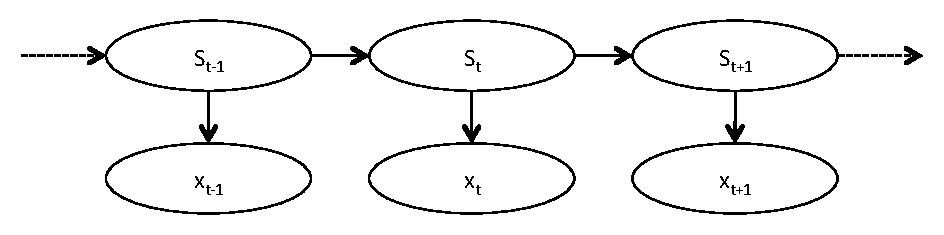
\includegraphics[width=0.65\textwidth]{HMM.pdf}
    \caption{Directed graph of a typical HMM}
    \label{fig:HMM:overview}
    \end{figure}

    \begin{itemize}
	\item A HMM is a \alert{doubly stochastic process}, explained with details in \cite{Zucchini:2009df}.
	\item The hidden states process $\{S_t \colon t = 1,2,\dots\}$ is a Markov chain:
		\[ \prob{S_t \mid \bS^{(t-1)}} = \prob{S_t \mid S_{t-1}},\ t = 2,3,\dots. \]
	\item The observed variable are conditionally distributed:
		\[ \prob{X_t \mid \bX^{(t-1)}, \bS^{(t-1)}} = \prob{X_t \mid S_t},\ t = 1,2,3,\dots. \]
	\end{itemize}
\end{frame}

%%%%%%%%%%%%%%%%%%%%

\subsection{Primary Statistics}

\begin{frame}[fragile,t]{Primary Statistics}
	\begin{itemize}
	\item State-dependent distribution (conditional distribution of $X$):
		\[ p_i(x) = \left \{ 
        \begin{array}{l l}
        \prob{X_t = x \mid S_t = i} & ,\text{if}\ X_t\ \text{is discrete,} \\
        f_t(x \mid S_t = i) & ,\text{if}\ X_t\ \text{is continuous.} \\
        \end{array} \right. \]
	\item Marginal distribution:
		\[ \prob{X_t = x} = \sum_{i=1}^{N} \prob{X_t = x \mid S_t = i}\prob{S_t = i} 
		= \sum_{i=1}^N p_i(x)\delta_i(t), \]
        or in form of matrix:
        \[ \begin{aligned}
		\prob{X_t = x} & = (\delta_1(t),\delta_2(t),\dots,\delta_N(t)) 
			\left ( \begin{array} {c c c}
				p_1(x) & & 0 \\
				& \ddots & \\
				0 & & p_N(x) \\
			\end{array} \right)
			\left ( \begin{array} {c}
				1 \\	\vdots \\	1 \\
			\end{array} \right) \\
		& = \bdelta(t)\bp(x)\one = \bpi\bGamma^{t-1}\bp(x)\one,
        \end{aligned} \]
    \end{itemize}
\end{frame}

\begin{frame}[fragile,t]{Primary Statistics}
    \begin{itemize}
    \item Likelihood:
		\[ L_T = \bpi\bp(x_1)\bGamma\bp(x_2)\bGamma\bp(x_3)\cdots\bGamma\bp(x_T)\one. \]
	\item Forward probabilities:
		\[ \begin{aligned}
		\balpha_t & = \bpi\bp(x_1)\bGamma\bp(x_2)\bGamma\bp(x_3)\cdots\bGamma\bp(x_t)
		= \bpi\bp(x_1)\prod_{s=2}^{t}\bGamma\bp(x_s),\\
		\alpha_t(j) & = \prob{\bX^{(t)} = \bx^{(t)}, S_t = j}.
		\end{aligned} \]
	\item Backward probabilities:
		\[ \begin{aligned}
		\bbeta_t & = \bGamma\bp(x_{t+1})\bGamma\bp(x_{t+2})\cdots\bGamma\bp(x_T)\one
		= \left(\prod_{s=t+1}^{T}\bGamma\bp(x_s)\right)\one, \\
		\beta_t(i) & = \prob{\bX^{(t+1:T)} = \bx^{(t+1:T)} \mid S_t = i},\ \prob{S_t = i}>0
		\end{aligned} \]
	\end{itemize}
\end{frame}

%%%%%%%%%%%%%%%%%%%%

\subsection{Expectation Maximization Algorithm}

\begin{frame}[fragile]{Expectation Maximization Algorithm}
	\begin{itemize}\vspace{0.4mm}
	\item Specifically known as Baum-Welch algorithm in the context of HMM,
		proposed separately in \cite{Baum:1966cy},\cite{Baum:1967gs} and \cite{Baum:1970do}.
	\item With forward and backward procedure, the algorithm has two steps:
		\begin{enumerate}
		\item \textbf{E step} calculates the expectations of (functions of) the missing data 
		conditional on the observations and the current estimate of $\btheta$;
		\item \textbf{M step} maximizes the CDLL w.r.t.\,$\btheta$.
		\end{enumerate}
	\item Essentially EM estimations are also a kind of \alert{MAP} estimation, 
		i.e.\,\alert{maximize a posterior} estimations.
	\end{itemize}
\end{frame}

\begin{frame}[fragile,t]{Expectation Maximization Algorithm}
	\begin{itemize}
	\item State value indicators:
		\[ u_j(t) = \left \{ \begin{array}{l l}
		1 & ,\text{iff}\ S_t = j \\
		0 & ,\text{otherwise}, \\
		\end{array} \right.
		\text{and}\ 
		v_{jk}(t) = \left \{ \begin{array}{l l}
		1 & ,\text{iff}\ S_{t-1} = j\ \text{and}\ S_t = k \\
		0 & ,\text{otherwise}. \\
		\end{array} \right. \]
	\item Maximize the complete-data log-likelihood (CDLL):
		\[ \begin{aligned}
		\log\left(\prob{\bx^{(T)},\bs^{(T)}}\right) & = 
		\underbrace{\sum_{j=1}^{N} u_j(1)\log\pi_j}_{\text{term 1}} + 
		\underbrace{\sum_{j=1}^{N}\sum_{k=1}^{N} 
			\left(\sum_{t=2}^Tv_{jk}(t)\right)\log\gamma_{jk}}_{\text{term 2}} \\ 
		& + \underbrace{\sum_{j=1}^{N}\sum_{t=1}^{T} u_j(t)\log p_j(x_t)}_{\text{term 3}}. 
		\end{aligned} \]
	\end{itemize}
\end{frame}

%%%%%%%%%%%%%%%%%%%%

\subsection{Prediction and Decoding}

\begin{frame}[fragile,t]{Prediction and Decoding}
	\begin{itemize}
	\item $h$-step forecast distribution:
		\[ \prob{X_{T+h} = x \mid \bX^{(T)} = \bx^{(T)}} = 
		\frac{\prob{\bX^{(T)} = \bx^{(T)}, X_{T+h} = x}}{\prob{\bX^{(T)} = \bx^{(T)}}} 
		= \frac{\balpha_T\bGamma^h\bp(x)\one}{\balpha_T\one}. \]
	\item Local decoding:
		\[ S_t^{\ast} = \argmax_{j = 1,2,\dots,N} \prob{S_t = j \mid \bX^{(T)} = \bx^{(T)}}. \]
	\item Global decoding:
		\[ \begin{aligned}
		\xi_{1i} & = \prob{S_1 = i,X_1 = x_1} = \pi_ip_i(x_1), \\
		\xi_{ti} & = \max_{s_1,s_2,\dots,s_{t-1}} 
			\prob{\bS^{(t-1)} = \bs^{(t-1)},S_t = i, \bX^{(T)} = \bx^{(T)}}, \\
		S_T & = \argmax_{i = 1,2,\dots,N} \xi_{Ti}, \\
		S_t & = \argmax_{i = 1,2,\dots,N} (\xi_{ti}\gamma_{i,S_{t+1}}).
		\end{aligned} \]
	\end{itemize}
\end{frame}

% !TEX encoding = UTF-8 Unicode

\section{\large Stock Return Series Prediction System}

%%%%%%%%%%%%%%%%%%%%

\subsection{System Overview}

\begin{frame}[fragile,t]{System Overview}
	\begin{figure}[!hbt]
    \center
    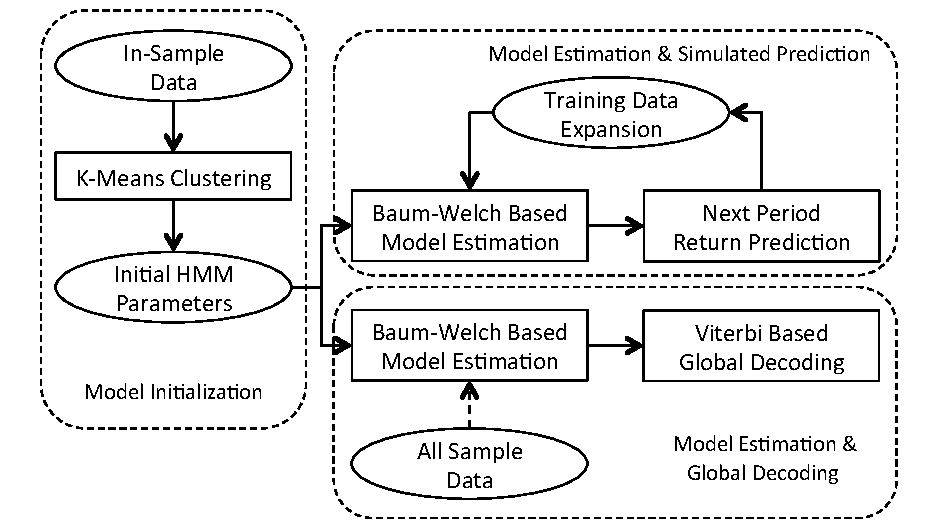
\includegraphics[width=0.85\textwidth]{system.pdf}
    \caption{Overview of the stock return series prediction system}
    \label{fig:system:overview}
    \end{figure}
\end{frame}

%%%%%%%%%%%%%%%%%%%%

\subsection{Model Initialization}

\begin{frame}[fragile,t]{Model Initialization}
	\begin{figure}[!hbt]
    \center
    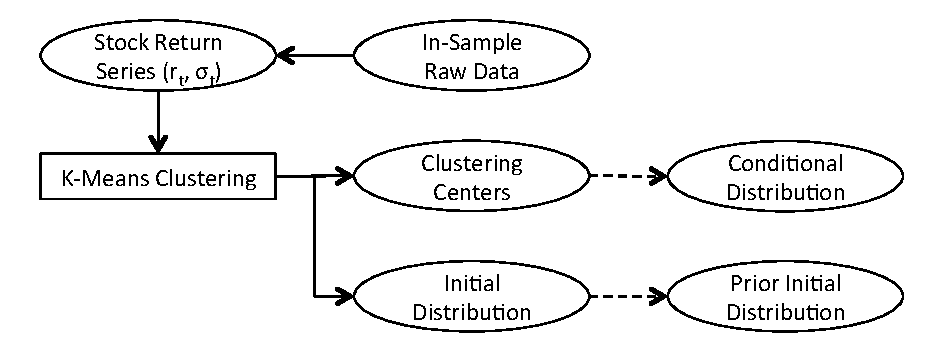
\includegraphics[width=0.8\textwidth]{initialization.pdf}
    \caption{Model initialization module}
    \label{fig:system:init}
    \end{figure}

    \begin{itemize}
    \item Transform the raw data into specified data structure (data tidying).
    \item Pre-process the raw data for observed variable series as K-Means input.
    \end{itemize}
\end{frame}

%%%%%%%%%%%%%%%%%%%%

\subsection{Simulated Prediction}

\begin{frame}[fragile,t]{EM-Based Model Estimation}
	\begin{figure}[!hbt]
    \center
    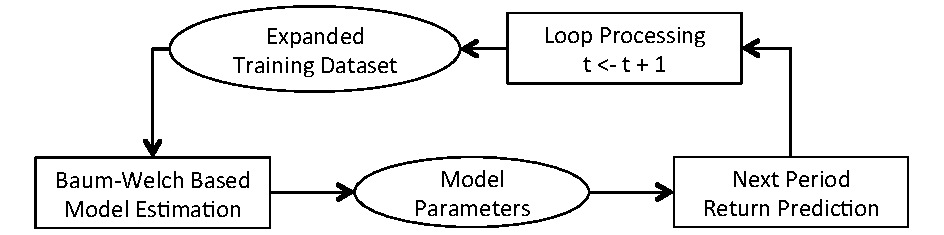
\includegraphics[width=0.8\textwidth]{EM.pdf}
    \caption{EM based model estimation procedure}
    \label{fig:system:EM}
    \end{figure}

    \begin{itemize}
    \item Carry out model estimation with EM algorithm (Baum-Welch).
    \item Calibrated parameters: hidden states initial distribution $\bpi$, 
    	hidden states final distribution $\bdelta$,
    	state transition matrix $\bGamma$, 
    	conditional distribution parameters $(\bmu,\bsigma)$.
    \item The model estimation procedure is \textit{adaptive}, 
    	i.e.\,it incorporates the new historical return information when the loop processes.
    \end{itemize}
\end{frame}

\begin{frame}[fragile,t]{Prediction}
    \begin{itemize}
    \item Two different ways to predict the \textit{price} of the next period:
    	\[ \begin{aligned}
		\text{static:}\ \hat{P}_t & = P_0 e^{\sum_{i=1}^{t}\hat{r}_i}, \\
		\text{adaptive:}\ \hat{P}_t & = P_{t-1} e^{\hat{r}_t},
		\end{aligned} \]
		where $P_{t-1}$ is the real price at time $t-1$ and 
		$P_0$ is the price of the first day when the prediction procedure begins.
    \item The first prediction procedure only considers the information of the returns, 
    	and thus the errors of predictions accumulate and are reflected on the predicted price.
    \item The second (so-called \alert{adaptive prediction}) procedure considers both the return and 
    	the \textit{price level} at $t-1$ to predict the price at $t$.
    \end{itemize}
\end{frame}

%%%%%%%%%%%%%%%%%%%%

\subsection{Global Decoding}

\begin{frame}[fragile,t]{Global Decoding}
	\begin{figure}[!hbt]
    \center
    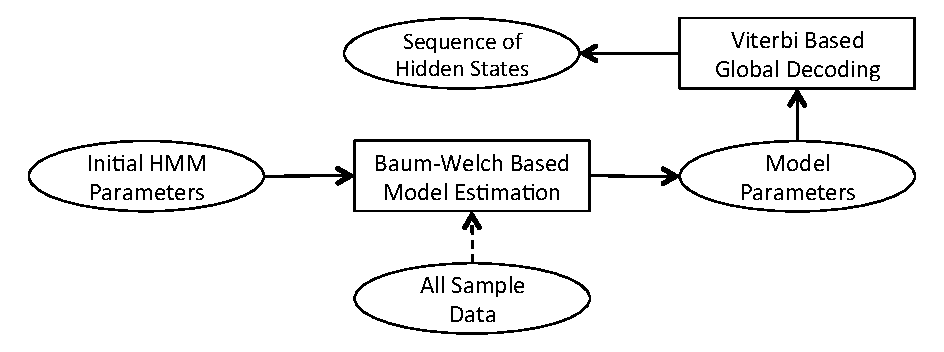
\includegraphics[width=0.8\textwidth]{decoding.pdf}
    \caption{Global decoding module}
    \label{fig:system:decoding}
    \end{figure}

    \begin{itemize}
    \item Independent with the simulated prediction module.
    \item Conduct Viterbi algorithm based global decoding to 
    	deduce the most probable sequence of hidden states during the observation period.
    \end{itemize}
\end{frame}
% !TEX encoding = UTF-8 Unicode

\section{\large Empirical Analysis}

%%%%%%%%%%%%%%%%%%%%

\subsection{Settings}

\begin{frame}[fragile,t]{Settings}
	\begin{itemize}\vspace{0.4mm}
	\item Stock returns conditional on the market states are normally distributed.
	\item Both Chinese and U.S.\.markets have and only have three hidden states,
        namely bear, intermediate and bull:
        \begin{enumerate}
        \item \textbf{Bear} means relatively low returns with high volatilities.
        \item \textbf{Intermediate} means returns and volatilities bot close to zero.
        \item \textbf{Bull} means relatively high returns with high volatilities.
        \end{enumerate}
        The number of hidden states is now artificially given and 
        will be analyzed and validated later.
    \item Some conjectures:
    	\begin{enumerate}
        \item Time lag effects exist and worsen due to too much weight of outdated information.
        \item Results may vary with observation periods and frequencies.
        \end{enumerate}
	\end{itemize}
\end{frame}

%%%%%%%%%%%%%%%%%%%%

\subsection{Chinese CSI 300 Index daily return series}

\subsubsection{Data Description}

\begin{frame}[fragile,t]{Chinese CSI 300 Index daily return series}
	\begin{figure}[!hbt]
    \center
    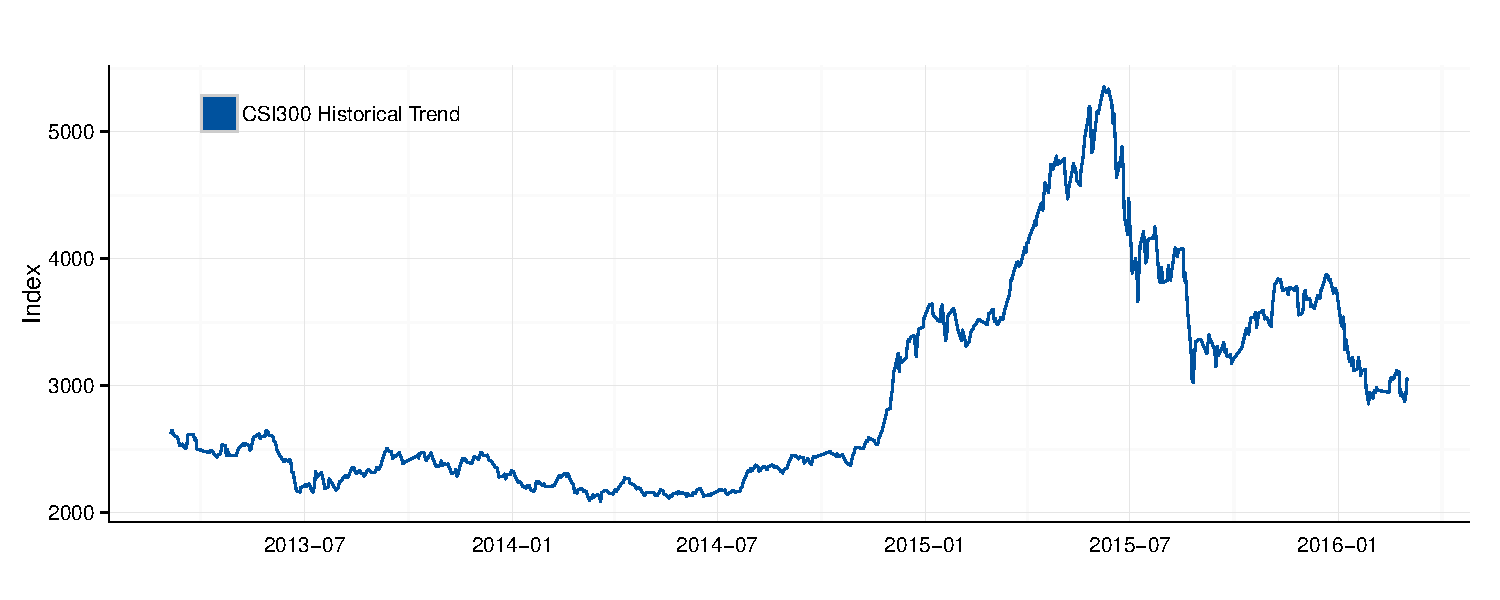
\includegraphics[width=0.8\textwidth]{daily/histFig1.pdf}
    \caption{CSI 300 historical prices}
    \label{fig:CSI:hist}
    \end{figure}

    \begin{itemize}
	\item Data range from Mar.\,$5^{th}$, 2013 to Mar\,$3^{rd}$, 2016, 
		729 prices within three years in total.
	\end{itemize}
\end{frame}

\subsubsection{Global Decoding Results}

\begin{frame}[fragile]{Chinese CSI 300 Index daily return series}
	\begin{figure}[!hbt]
    \center
    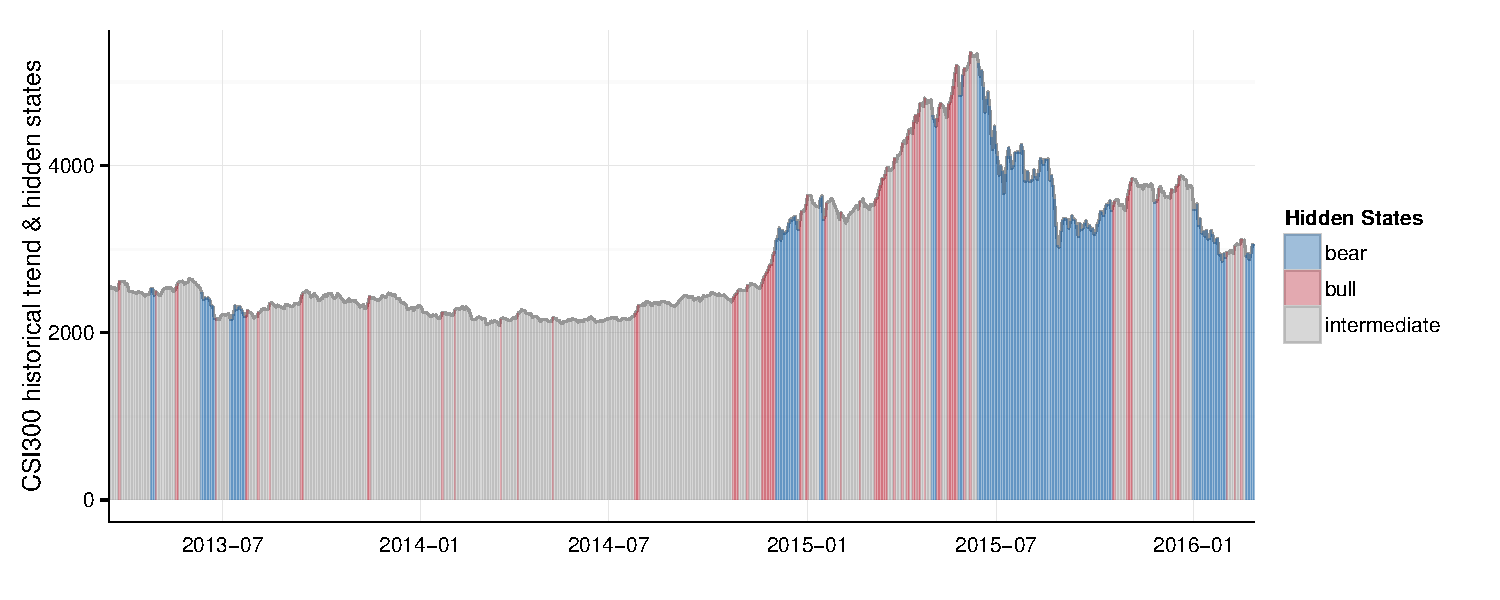
\includegraphics[width=\textwidth]{daily/statesFig1.pdf}
    \caption{CSI 300 in-sample trend and states sequence}
    \label{fig:CSI:seqstates}
    \end{figure}
\end{frame}

\begin{frame}[fragile]{Chinese CSI 300 Index daily return series}
	\begin{figure}[!hbt]
    \center
    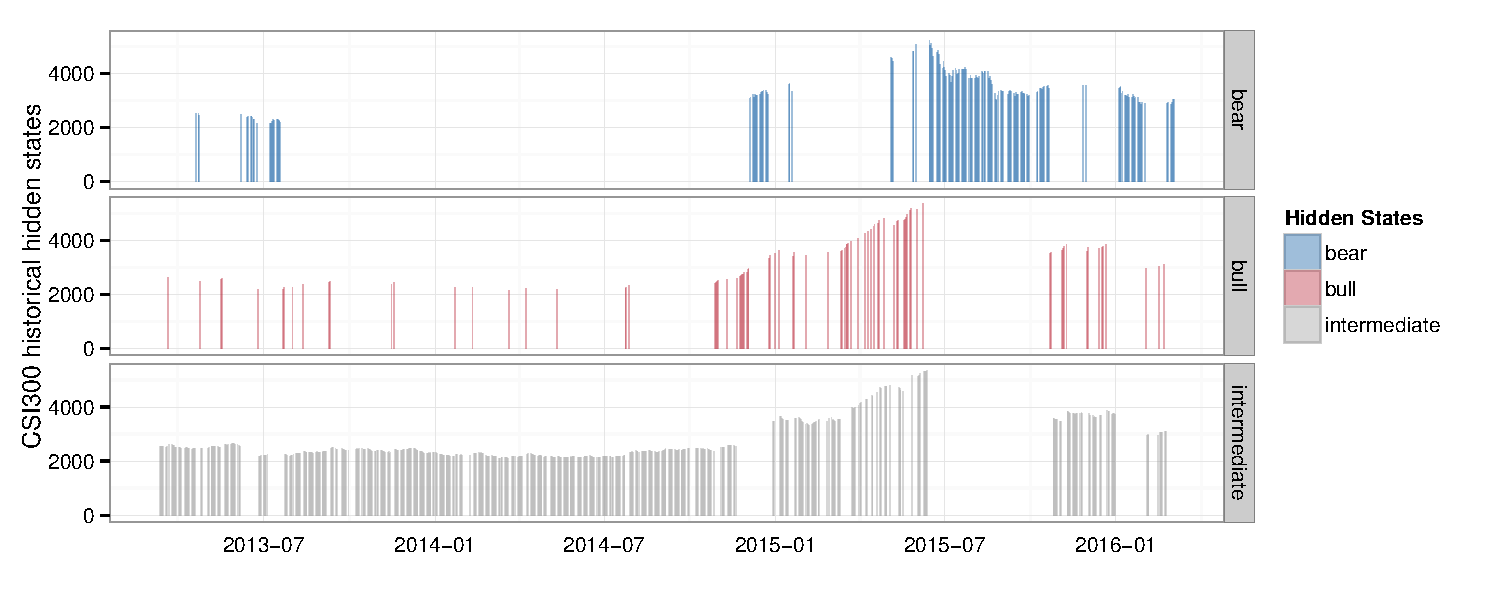
\includegraphics[width=\textwidth]{daily/statesFig2.pdf}
    \caption{CSI 300 historical hidden states}
    \label{fig:CSI:states}
    \end{figure}
\end{frame}

\subsubsection{State Transition Matrix}

\begin{frame}[fragile,t]{Chinese CSI 300 Index daily return series}
	\begin{figure}[!hbt]
    \center
    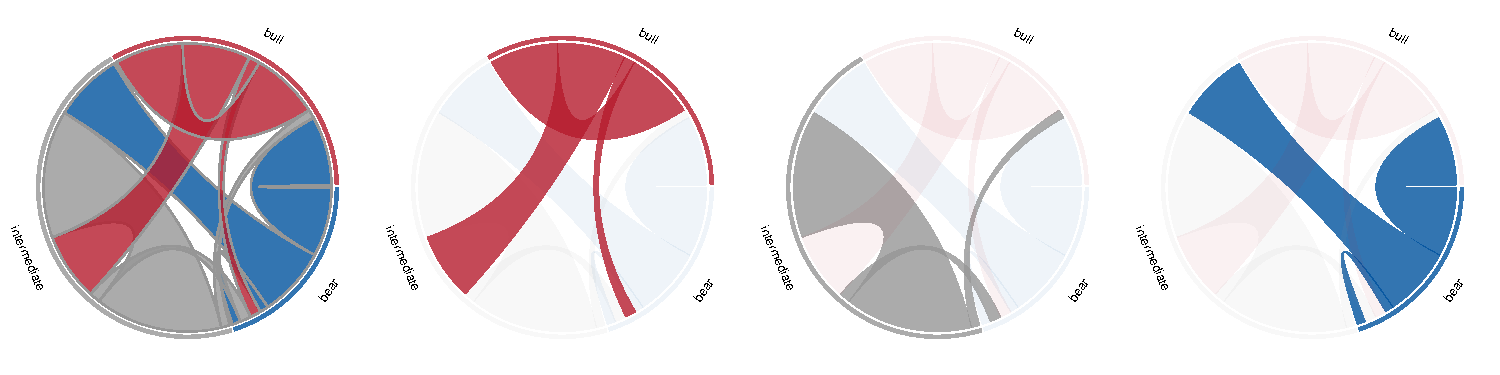
\includegraphics[width=\textwidth]{daily/transFig1.pdf}
    \caption{State transition for CSI 300 in-sample data}
    \label{fig:CSI:transition}
    \end{figure}

    \only<1>{
    \vspace*{-0.1cm}
    \begin{itemize}
	\item Colored chords start from the (same) color to another color 
		represent the transition probabilites.
	\item The thickness of the chords represent the relative relationships among the probabilities.
	\end{itemize}}
	\only<2>{
	\begin{exampleblock}{Example (Part 1 \& 2 of Fig.\,\ref{fig:CSI:transition})}
	There is a red chord starting from bull (red) and ending with intermediate (grey). 
	It represents the probability that the bull transits into the intermediate.
	Red to grey is the thickest, meaning it is most likely for bull to go into the intermediate.
	\end{exampleblock}}
\end{frame}

\begin{frame}[fragile]{Chinese CSI 300 Index daily return series}
	\begin{figure}[!hbt]
    \center
    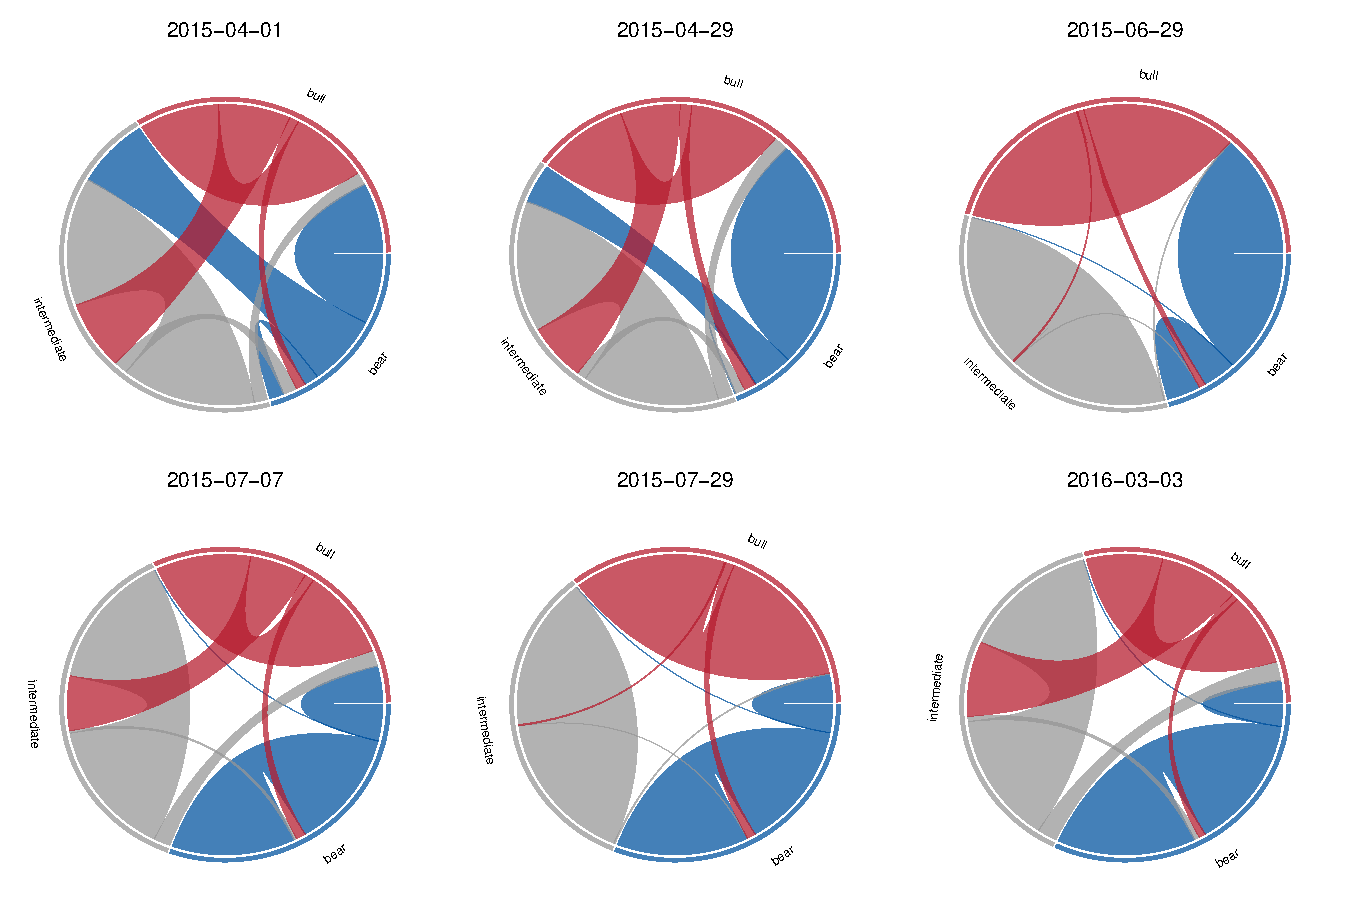
\includegraphics[width=0.75\textwidth]{daily/transFig3.pdf}
    \caption{Typical state transition matrices during the entire period }
    \label{fig:CSI:transitiontypical}
    \end{figure}
\end{frame}

\subsubsection{Conditional Distribution Parameters}

\begin{frame}[fragile,t]{Chinese CSI 300 Index daily return series}
	\begin{figure}[!hbt]
    \center
    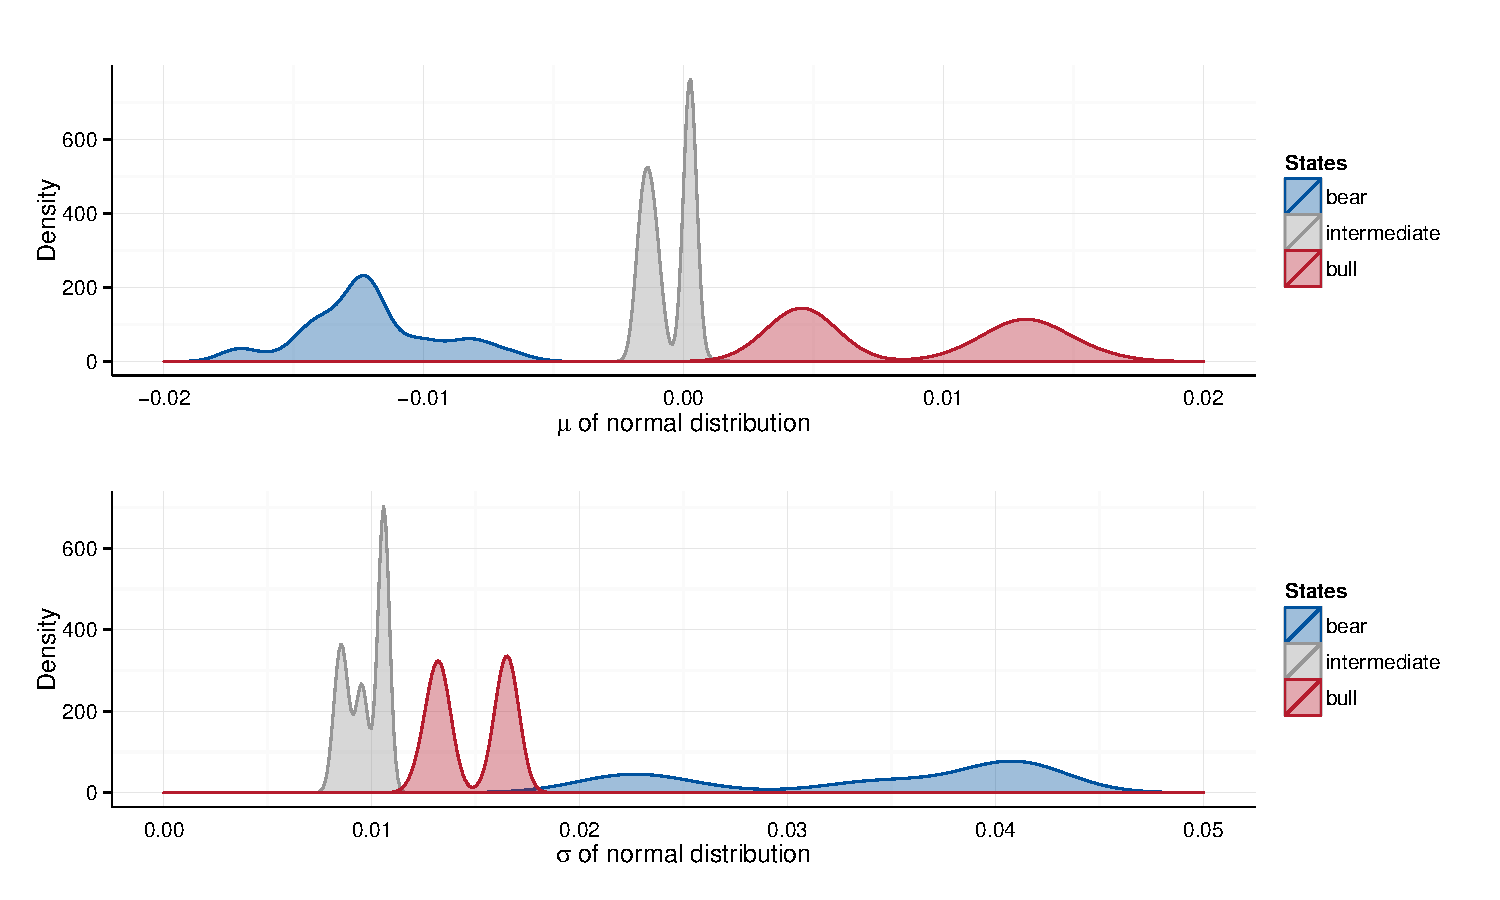
\includegraphics[width=0.72\textwidth]{daily/paramFig2.pdf}
    \caption{Density distribution of conditional distribution parameters}
    \label{fig:CSI:distdist}
    \end{figure}

    \vspace*{-1em}
	\begin{itemize}
	\item Conditional distribution parameters change with time goes by.
	\end{itemize}   
\end{frame}

\subsubsection{Simulated Predictions}

\begin{frame}[fragile,t]{Chinese CSI 300 Index daily return series}
	\begin{figure}[!hbt]
    \center
    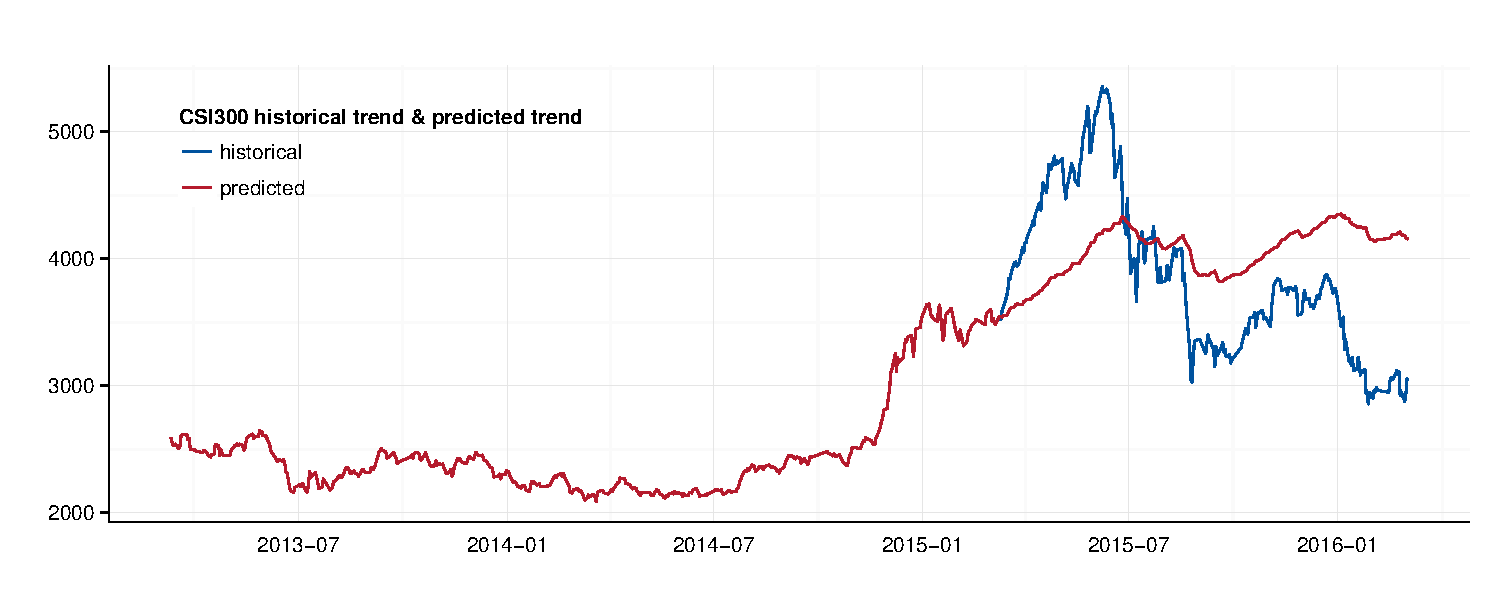
\includegraphics[width=\textwidth]{daily/predictionFig1.pdf}
    \caption{CSI 300 simulated prediction result}
    \label{fig:CSI:predictionall}
    \end{figure}

    \begin{itemize}
	\item Errors accumulate for long-period static predictions and time lag effects exist.
	\end{itemize}   
\end{frame}

\begin{frame}[fragile]{Chinese CSI 300 Index daily return series}
	\begin{figure}[!hbt]
    \center
    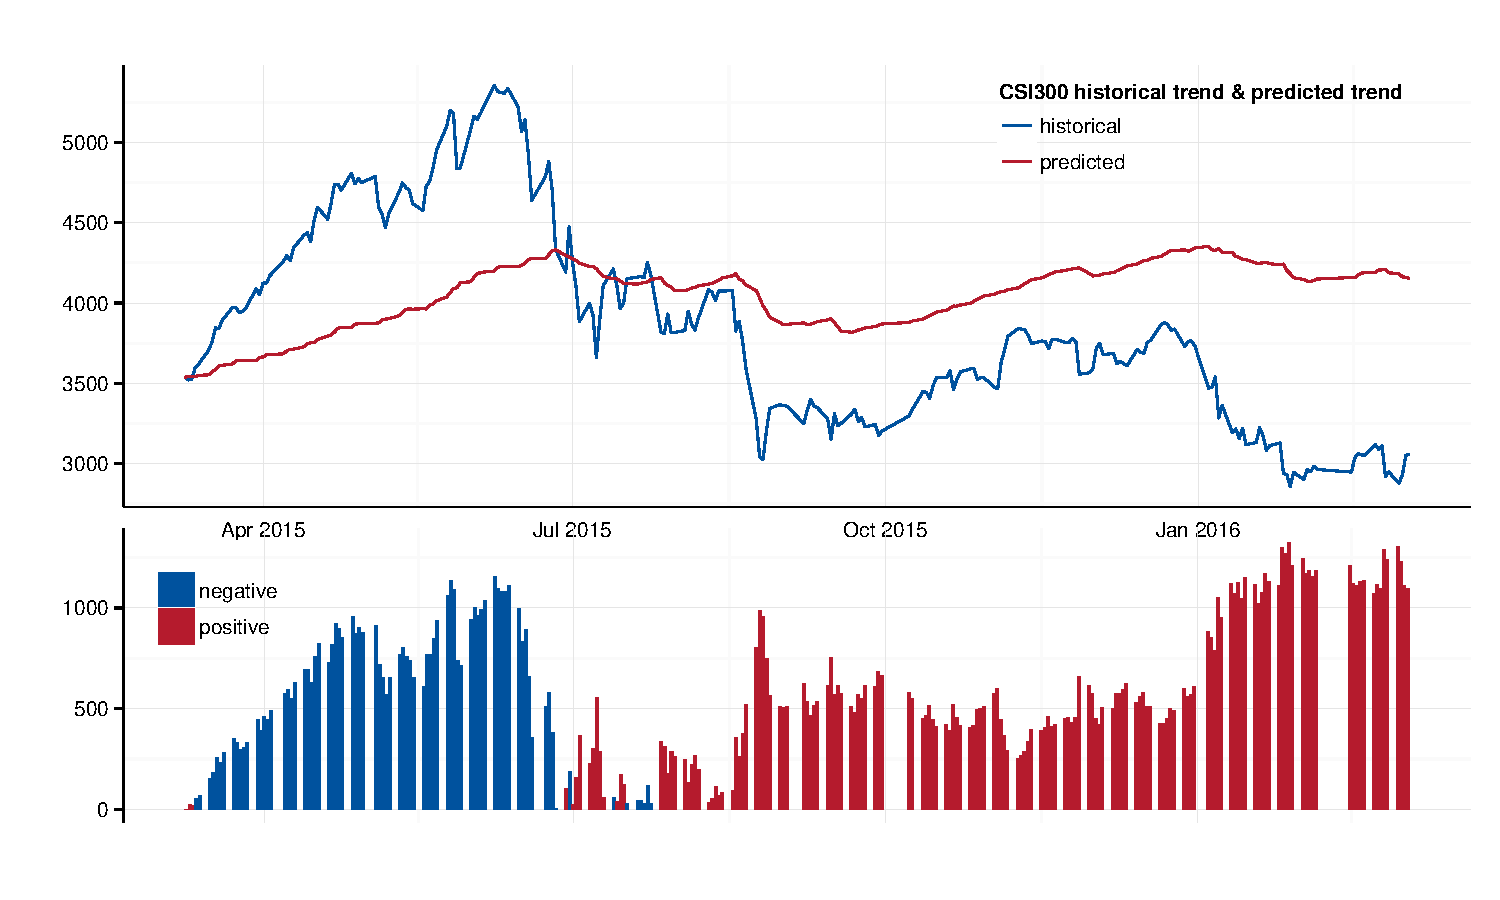
\includegraphics[width=0.8\textwidth]{daily/predictionFig2.pdf}
    \caption{CSI 300 simulated prediction result out-of-sample part}
    \label{fig:CSI:predictionout}
    \end{figure}
\end{frame}

\begin{frame}[fragile]{Chinese CSI 300 Index daily return series}
	\begin{figure}[!hbt]
    \center
    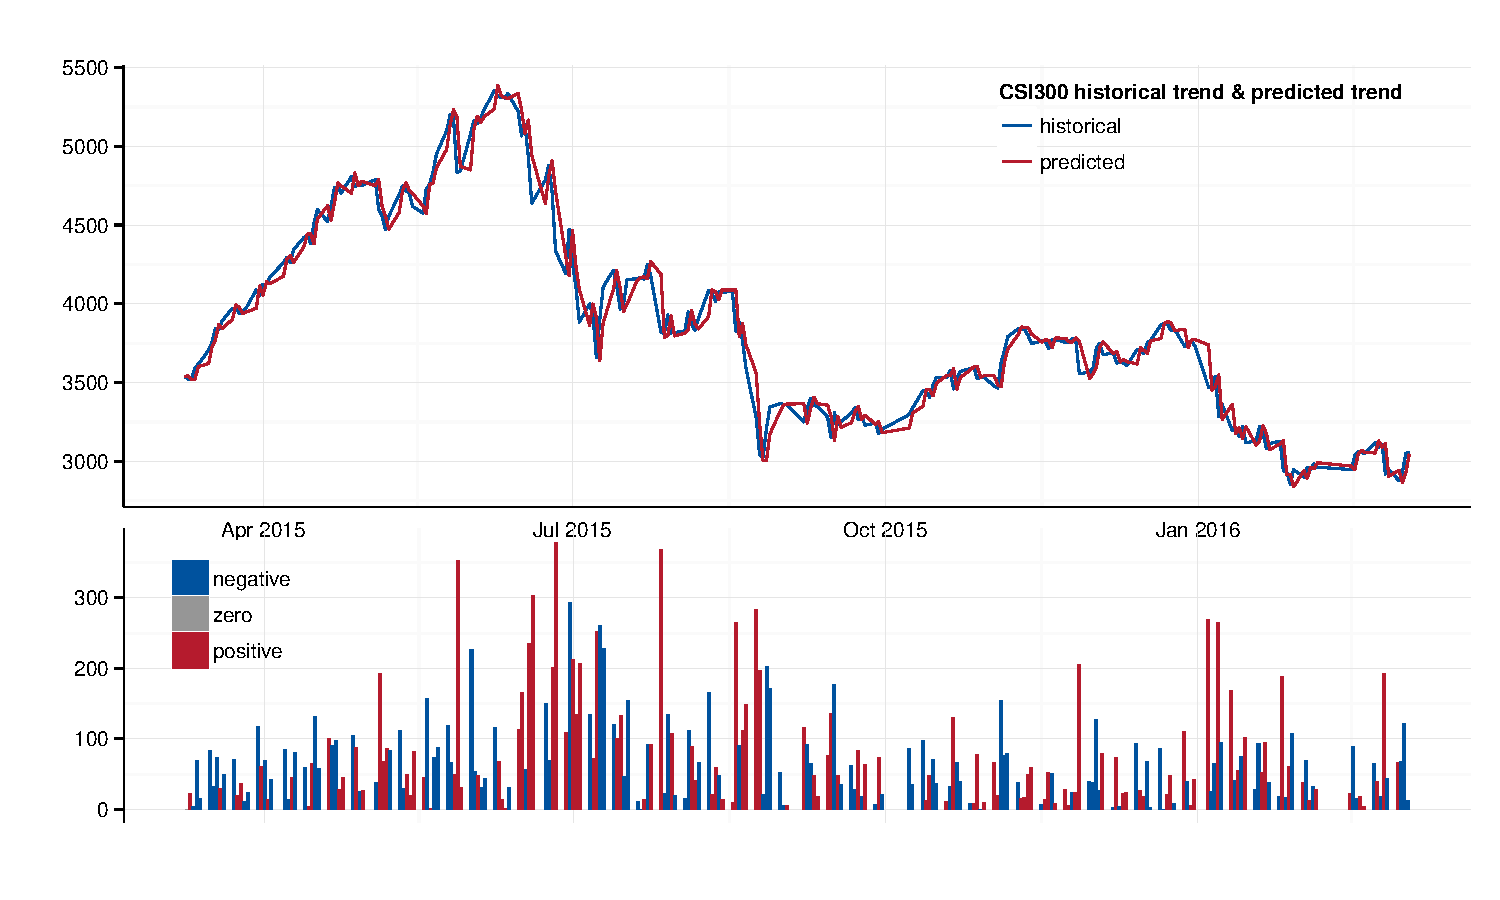
\includegraphics[width=0.8\textwidth]{daily/predictionFig4.pdf}
    \caption{CSI 300 adaptive predictions}
    \label{fig:CSI:adaptive}
    \end{figure}
\end{frame}

\begin{frame}[fragile,t]{Chinese CSI 300 Index daily return series}
	\begin{figure}[!hbt]
    \center
    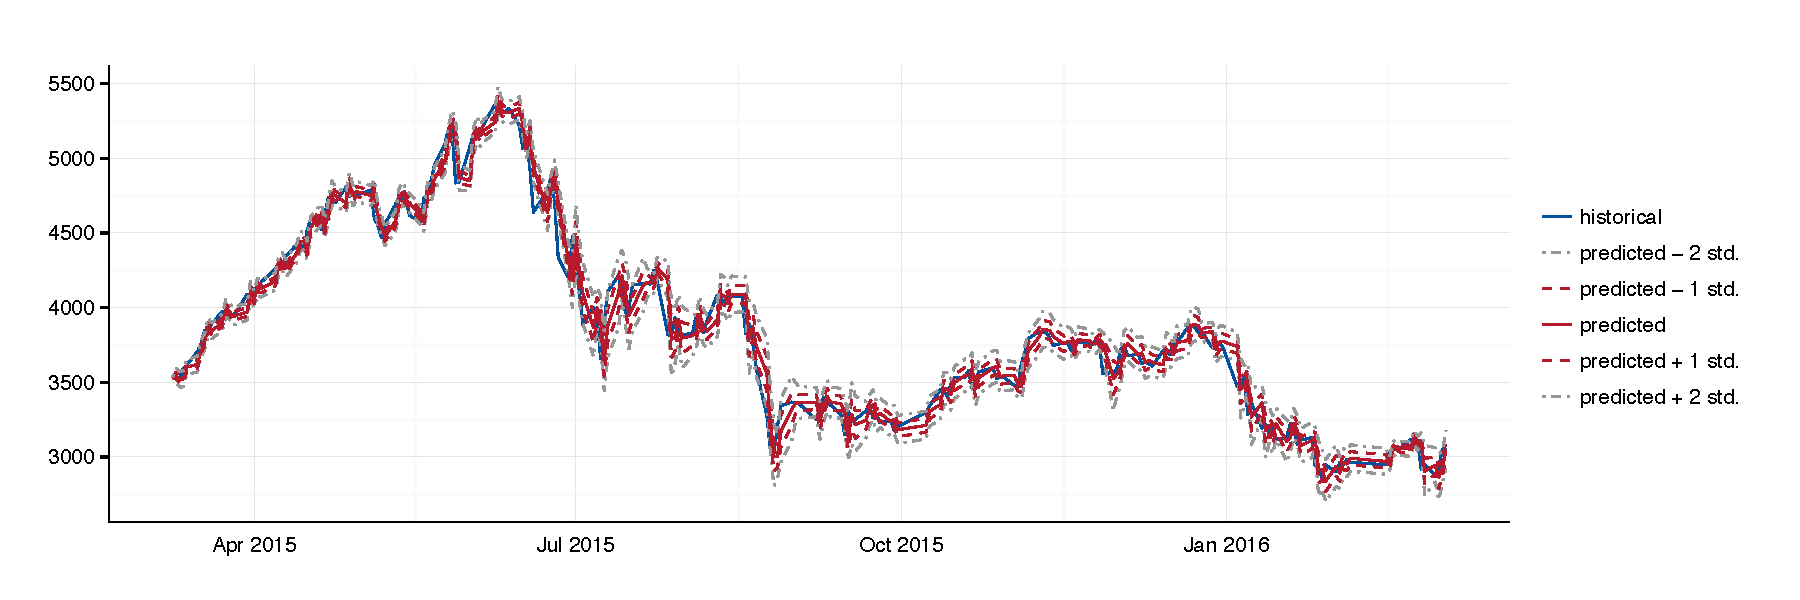
\includegraphics[width=\textwidth]{daily/predictionFig5.pdf}
    \caption{CSI 300 adaptive predictions with confidence interval}
    \label{fig:CSI:adaptiveconfi}
    \end{figure}

    \begin{itemize}
	\item All actual historical returns are within two standard deviations from the predicted return,
		and thus the adaptive predicted price level.
	\end{itemize}   
\end{frame}

%%%%%%%%%%%%%%%%%%%%

\subsection{The Number of Hidden States}

\begin{frame}[fragile,t]{The Number of Hidden States}
	\begin{figure}[!hbt]
    \begin{center}
    \subfigure[AIC vs. N]
        {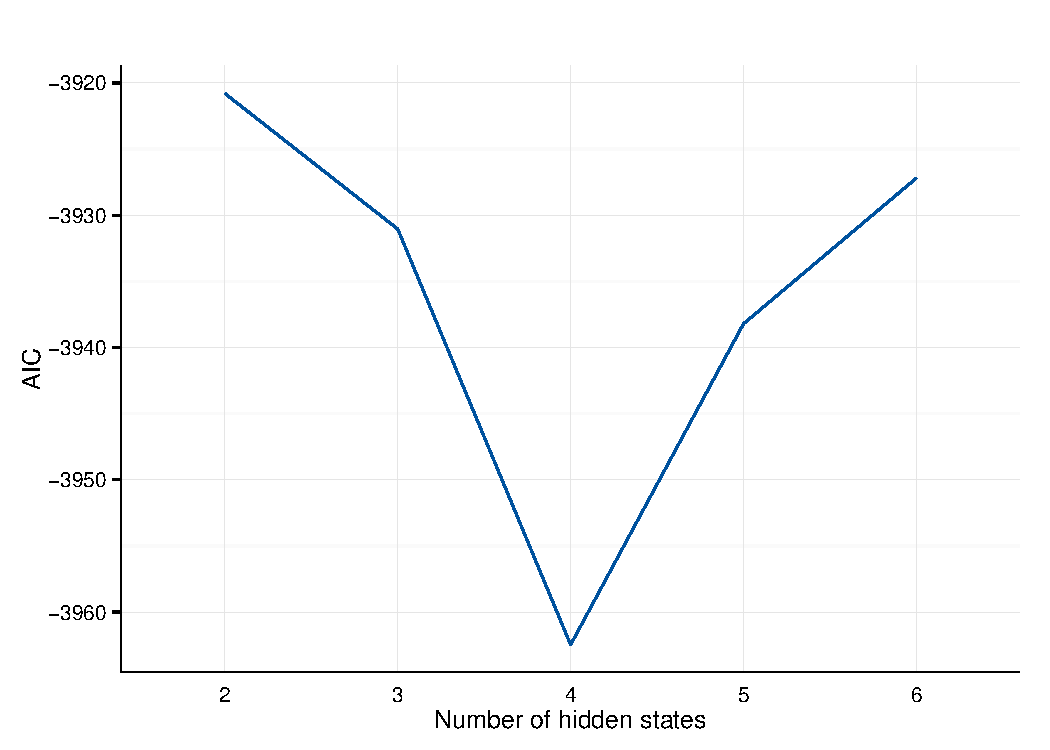
\includegraphics[width=0.45\textwidth]{states/numStateAIC.pdf}}
    \subfigure[BIC vs. N]
        {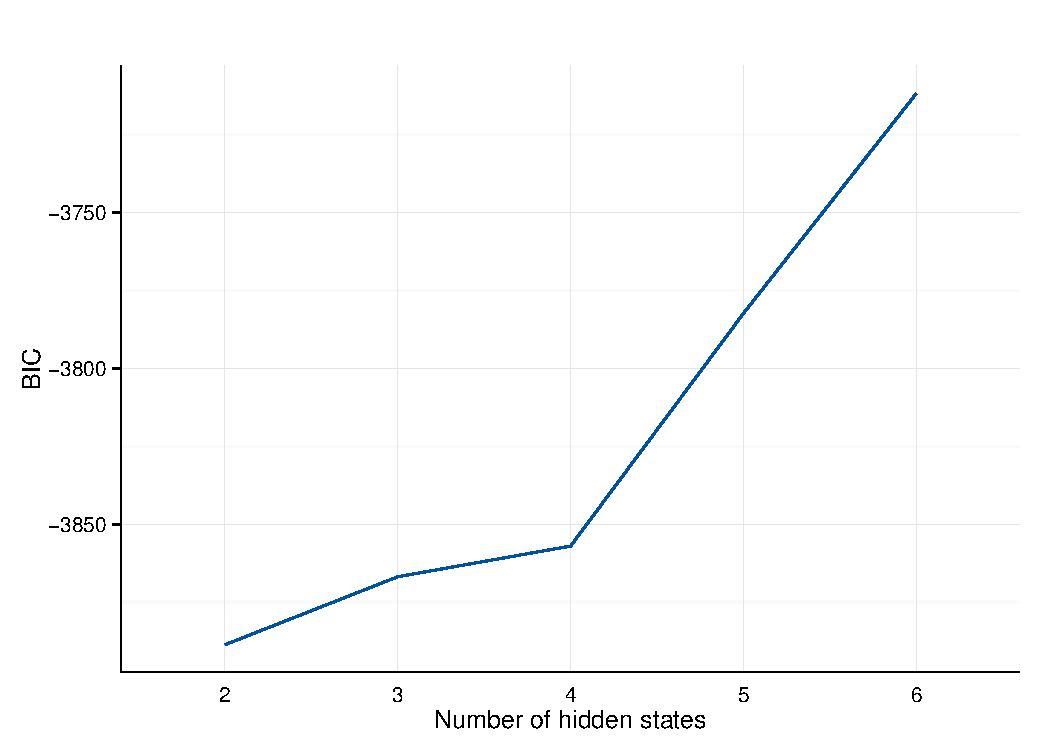
\includegraphics[width=0.45\textwidth]{states/numStateBIC.pdf}}
    \end{center}
    \caption{Goodness of fit for different number of hidden states}
    \label{fig:result:states}
    \end{figure}

    \vspace*{-1em}
    \begin{itemize}
	\item Four is optimal from AIC and two from BIC, so three is reasonable.
	\end{itemize}
\end{frame}

%%%%%%%%%%%%%%%%%%%%

\subsection{Prediction Results Summary}

\begin{frame}[fragile]{Prediction Results Summary}
	\begin{table}[!hbt]
    \center
    \caption{Brief description of all prediction results}
    \label{table:results}
    \begin{tabular}{c c c c c}
    \hline
    Target Index  &  Data Frequency  &  Time Period  &  Data Length  &  Win Ratio  \\
    \hline
    S\&P 500  &  daily  &  2013$\sim$2016  &  757  &  50.4\%  \\
    CSI 300   &  daily  &  2013$\sim$2016  &  729  &  50.2\%  \\
    CSI 300   &  60min  &  2013$\sim$2014  &  968  &  51.7\%  \\
    CSI 300   &  60min  &  2014$\sim$2015  &  976  &  55.5\%  \\
    CSI 300   &  60min  &  2015$\sim$2016  &  972  &  50.5\%  \\
    CSI 300   &  10min  &  2013$\sim$2014  &  5808  &  51.7\%  \\
    CSI 300   &  10min  &  2014$\sim$2015  &  5856  &  57.5\%  \\
    CSI 300   &  10min  &  2015$\sim$2016  &  5832  &  52.0\%  \\
    \hline
    \end{tabular}
    \end{table}
\end{frame}

% !TEX encoding = UTF-8 Unicode

\section{\large Summary}

%%%%%%%%%%%%%%%%%%%%

\subsection{Conclusion}

\begin{frame}[fragile,t]{Conclusion}
	\begin{block}{For the System}
    \begin{itemize}
    \item The system is complete, encapsulated and user-friendly.
    \item The system performs well in adaptive predictions, 
    	all actual returns fall in the $95.45\%$ confidence interval.
    \item Time lag effects exist, so sample reweighting is necessary to improve the performance.
    \end{itemize}
    \end{block}
    
    \begin{block}{For Empirical Analyses}
    \begin{itemize}
    \item Data populations with longer observation periods tend to 
    	provide more accurate hidden states anlysis results then short-term data.
    \item Data populations with higher observation frequencies
		tend to outperform those with lower frequencies w.r.t.\,prediction.
    \end{itemize}
    \end{block}
\end{frame}

%%%%%%%%%%%%%%%%%%%%

\subsection{Future Work}

\begin{frame}[fragile,t]{Future Work}
	\begin{block}{Time Lag Effects}
    \begin{itemize}
    \item \textbf{Rolling window method}, more popular in the industry,
    	the size of the window should be optimized.
    \item \textbf{Exponential weighted expectation maximization (EWEM) algorithm},
    	proposed in \cite{Zhang:2005tp}, more complex to implement.
    \end{itemize}
    \end{block}
    
    \begin{block}{Particle Filter}
    \begin{itemize}
    \item Standard tool for HMM estimation when the latent variable is continuous,
    	one of the most famous cases being Kalman filter.
    \item PF can incorporates economic meanings into values of the latent variable while currently 
    	we only consider the hidden states as categorical.
    \end{itemize}
    \end{block}
\end{frame}

%%%%%%%%%%%%%%%%%%%%%%%%%%

\appendix

\section*{\large Appendix}
% !TEX encoding = UTF-8 Unicode
\scriptsize

\begin{frame}[fragile,t]{Full Presentation of CSI 300 Results Visualization}
	\begin{figure}[!hbt]
    \center
    \subfigure[CSI 300 daily index]
        {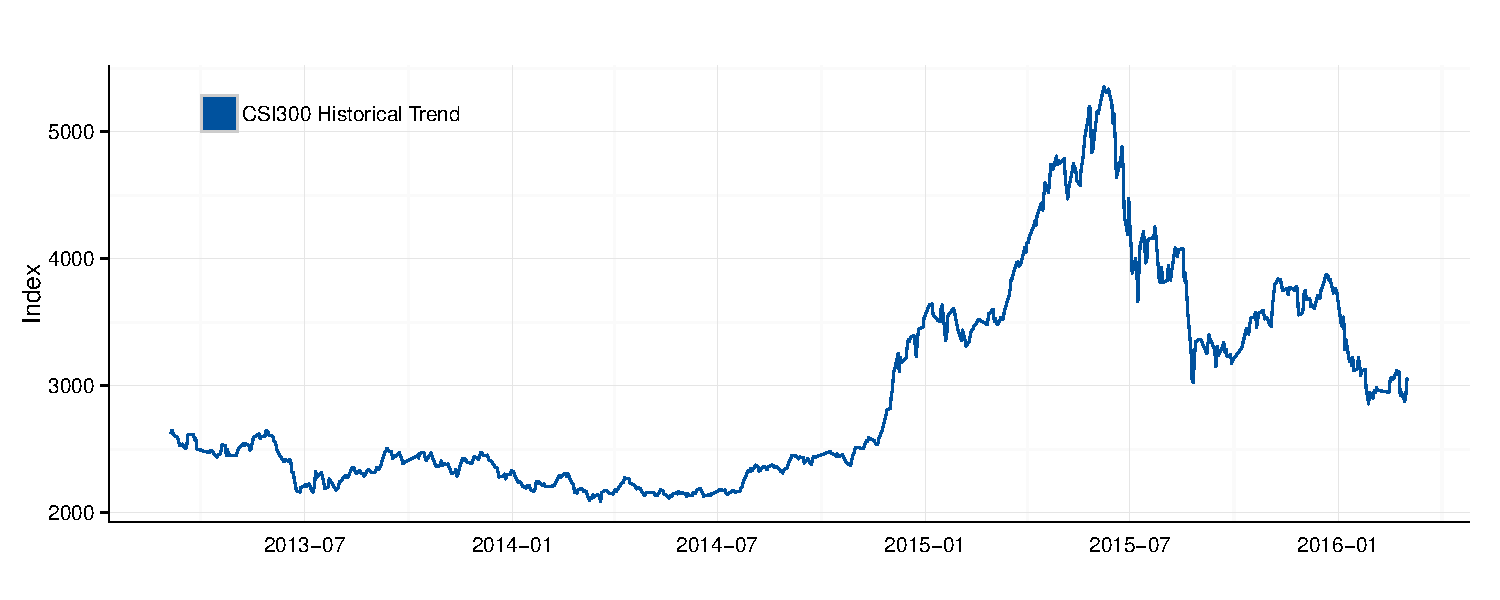
\includegraphics[width=0.48\textwidth]{daily/histFig1.pdf}}
    \subfigure[Daily returns and K-Means states]
        {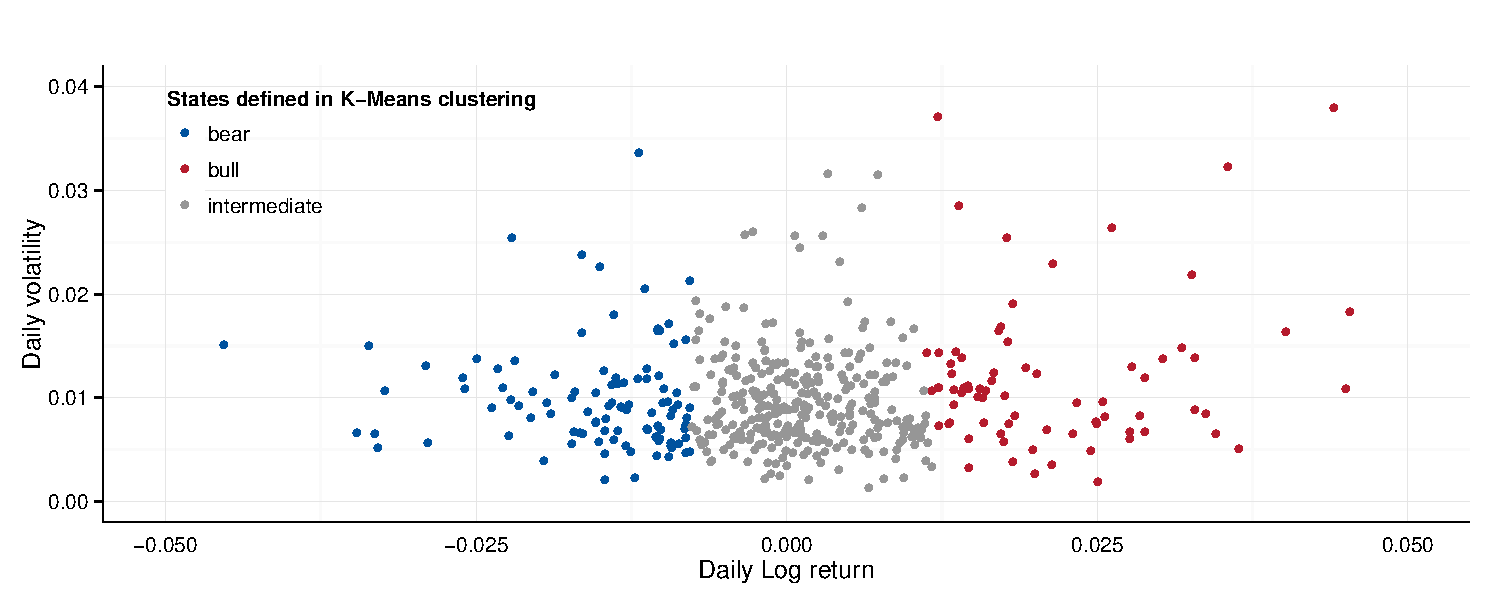
\includegraphics[width=0.48\textwidth]{daily/histFig2.pdf}}
    \subfigure[Daily returns distribution]
        {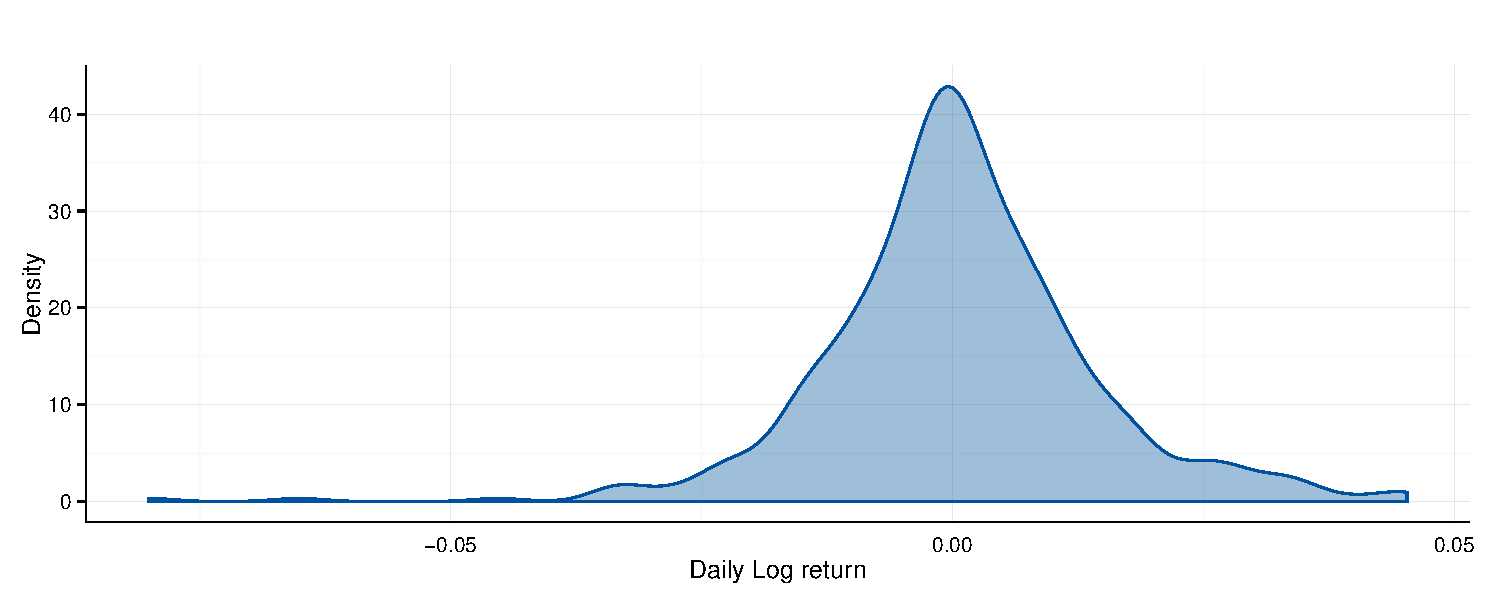
\includegraphics[width=0.48\textwidth]{daily/histFig4.pdf}}
    \subfigure{\hspace{0.47\textwidth}}
    \caption{Data description}
    \end{figure}
\end{frame}

\begin{frame}[fragile,t]{Full Presentation of CSI 300 Results Visualization}
	\begin{figure}[!hbt]
    \center
    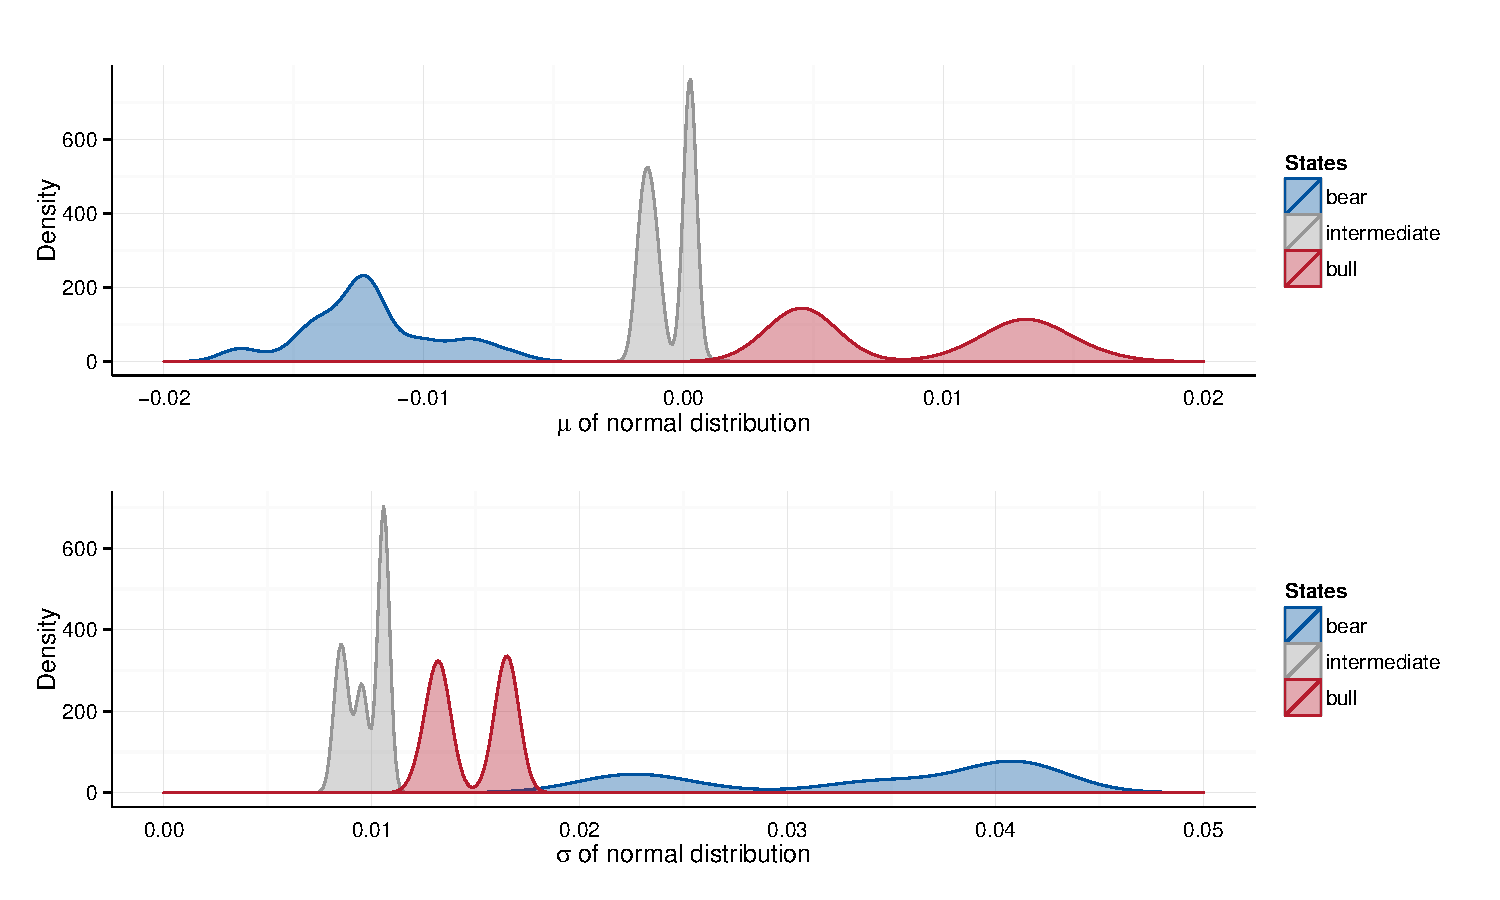
\includegraphics[width=0.82\textwidth]{daily/paramFig2.pdf}
    \caption{Density distribution of conditional distribution parameters}
    \end{figure}
\end{frame}

\begin{frame}[fragile,t]{Full Presentation of CSI 300 Results Visualization}
	\begin{figure}[!hbt]
    \center
    \subfigure[Historical index and states]
        {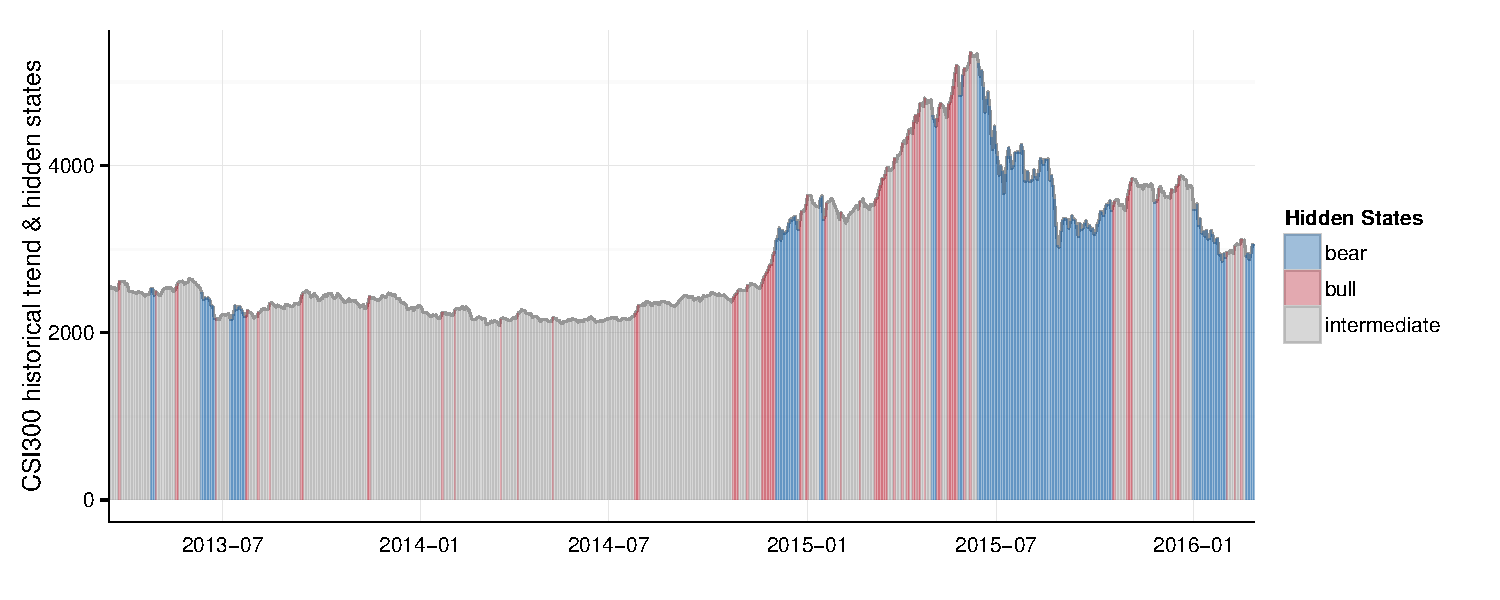
\includegraphics[width=0.49\textwidth]{daily/statesFig1.pdf}}
    \subfigure[Hidden states facets]
        {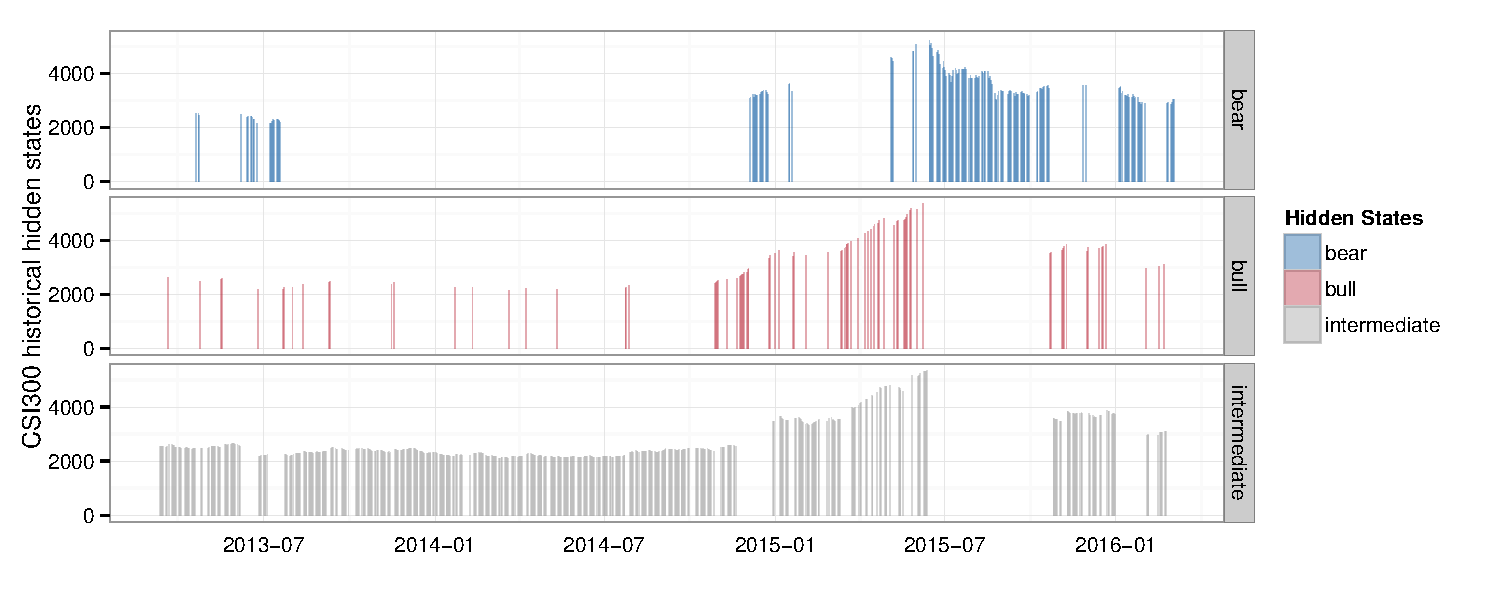
\includegraphics[width=0.49\textwidth]{daily/statesFig2.pdf}}
    \subfigure[HMM and K-Means states comparison]
        {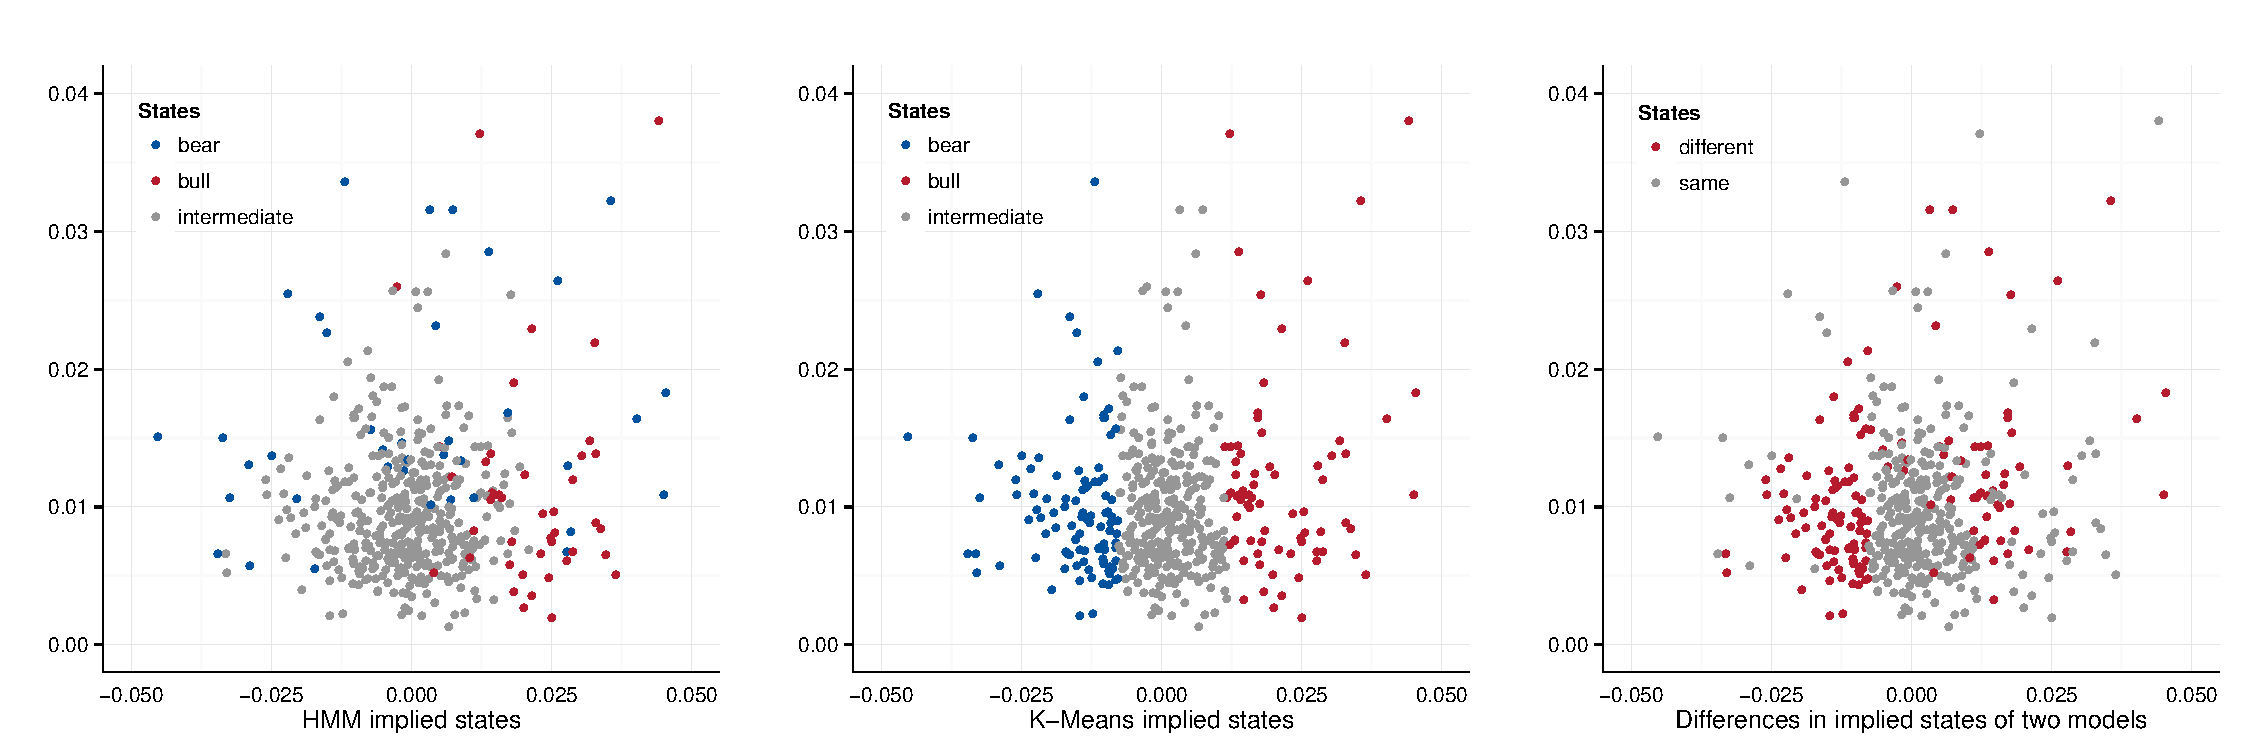
\includegraphics[width=0.51\textwidth]{daily/statesFig3.pdf}}
    \subfigure{\hspace{0.47\textwidth}}
    \caption{Historical hidden states results}
    \end{figure}
\end{frame}

\begin{frame}[fragile,t]{Full Presentation of CSI 300 Results Visualization}
	\begin{figure}[!hbt]
	\center
	\hspace*{-0.45cm}
	\subfigure[Simulated prediction result]
	    {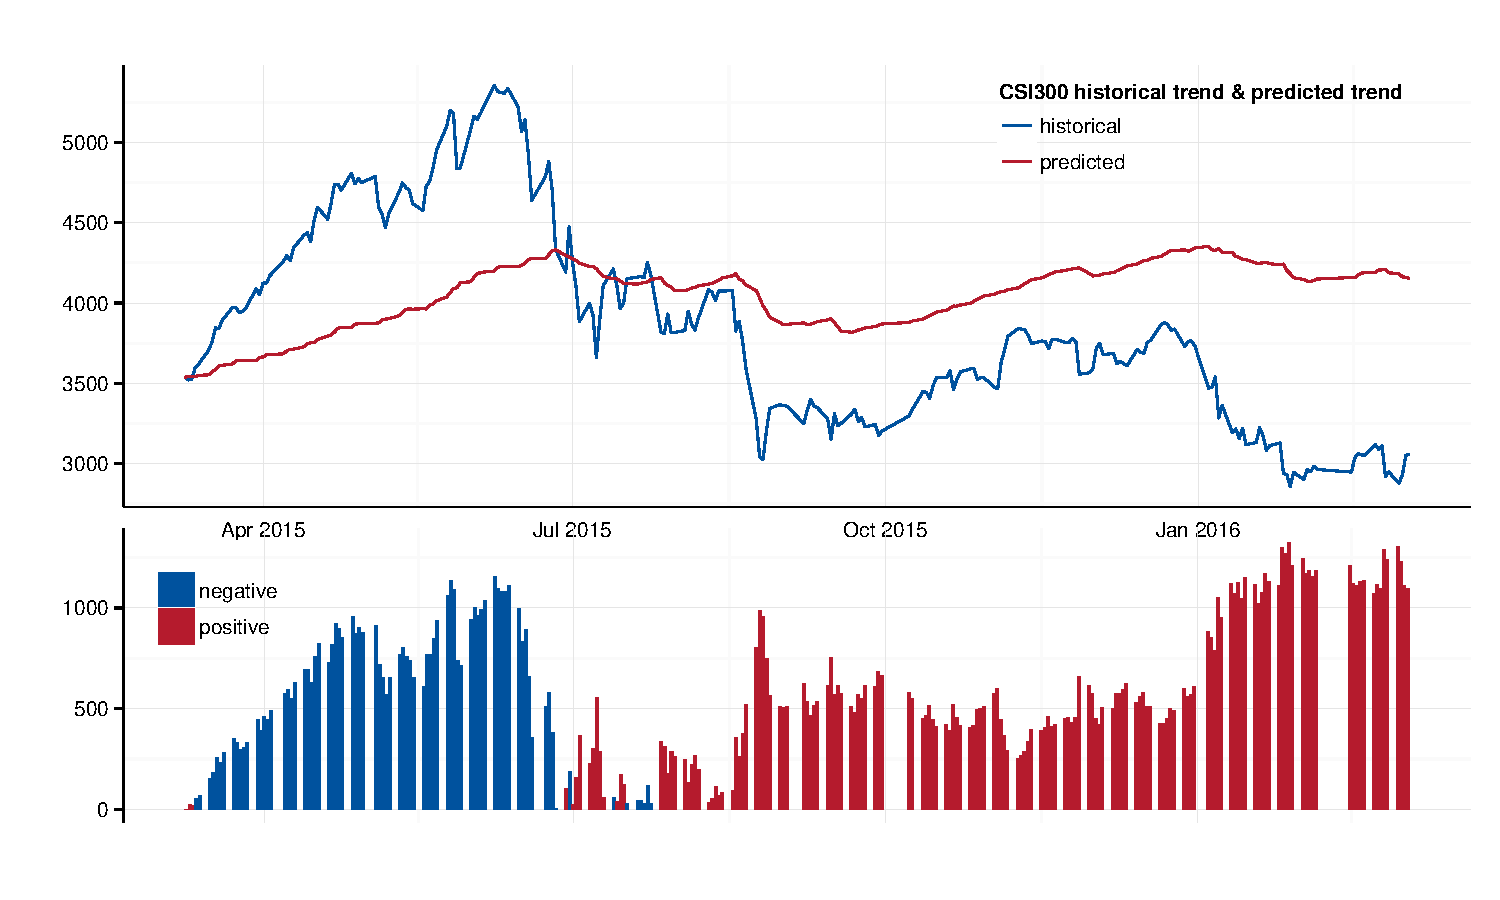
\includegraphics[width=0.44\textwidth]{daily/predictionFig2.pdf}}
	\hspace{1cm}
	\subfigure[Adaptive prediction result]
	    {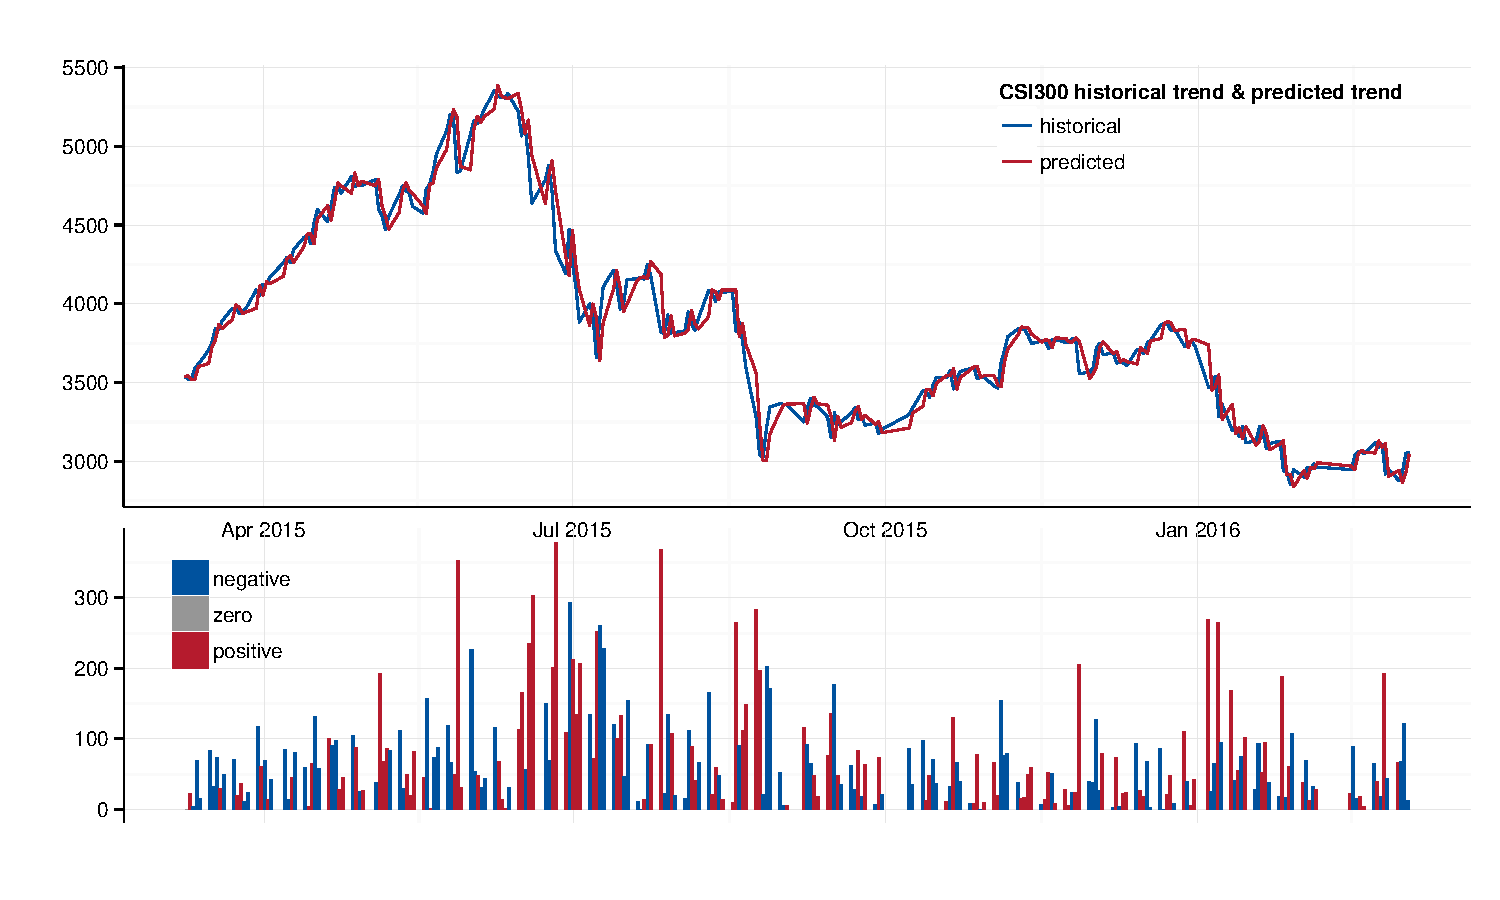
\includegraphics[width=0.44\textwidth]{daily/predictionFig4.pdf}}
	\subfigure[Simulated prediction with confidence band]
	    {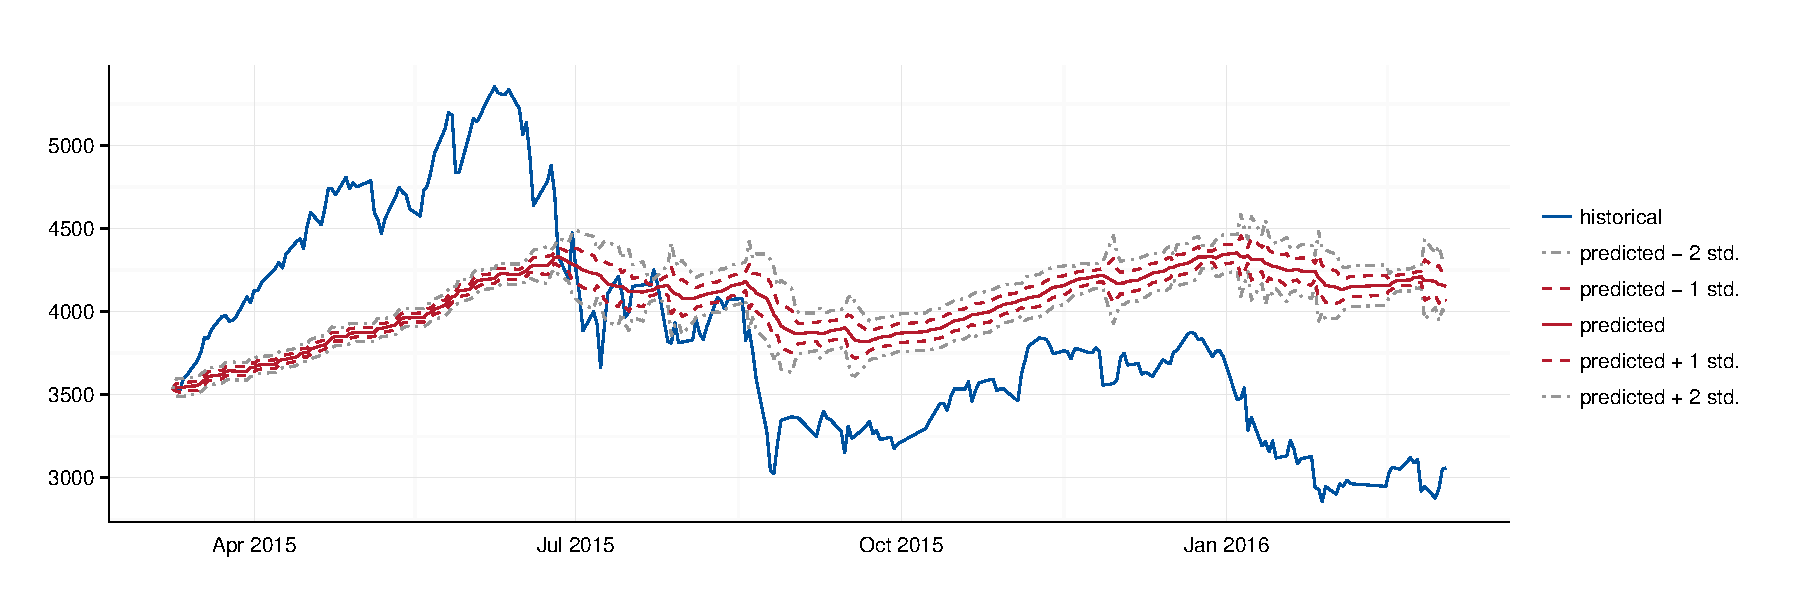
\includegraphics[width=0.45\textwidth]{daily/predictionFig3.pdf}\hspace*{0.5cm}}
	\subfigure[Adaptive prediction with confidence band]
	    {\hspace*{0.5cm}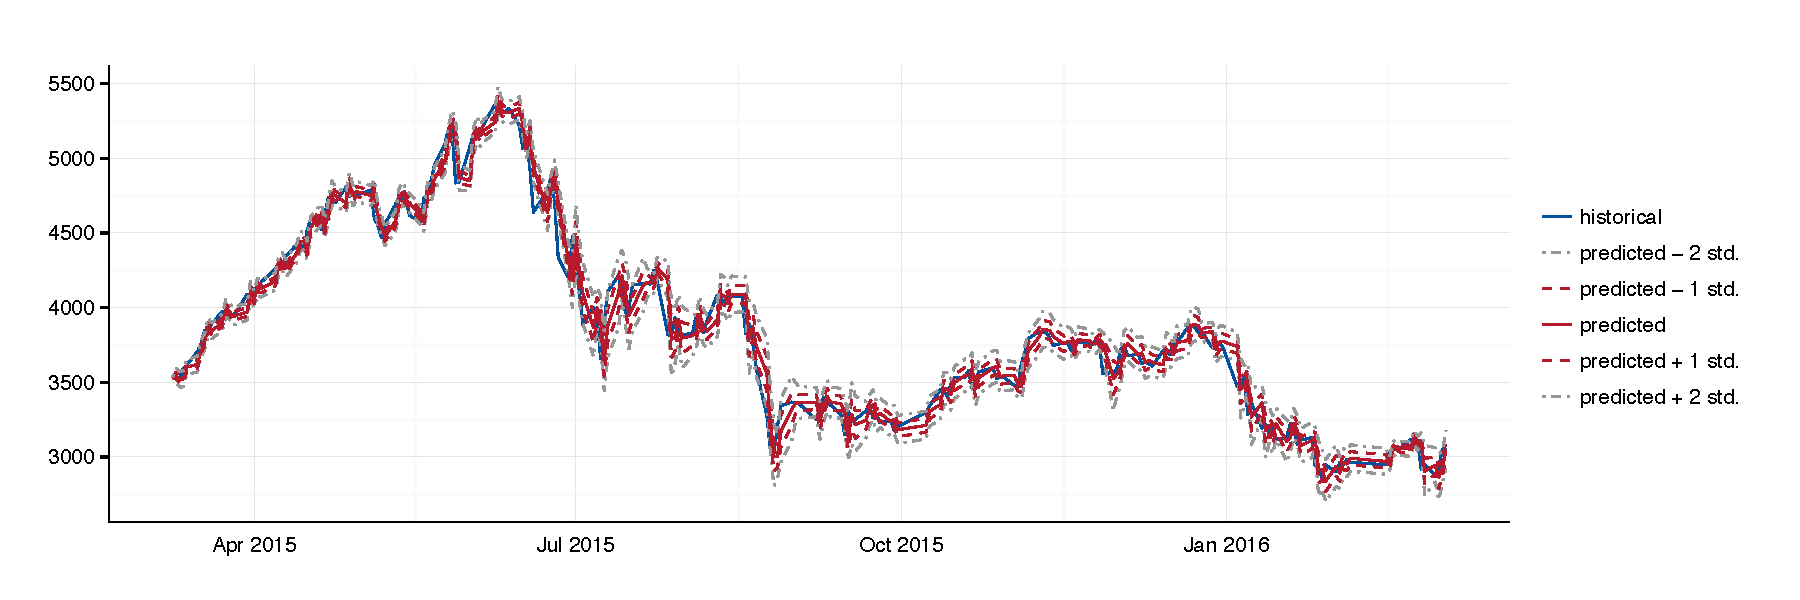
\includegraphics[width=0.45\textwidth]{daily/predictionFig5.pdf}}
	\caption{Simulated prediction results}
	\label{fig:app:daily:prediction}
	\end{figure}
\end{frame}









%%%%%%%%%%%%%%%%%%%%%%%%%%

\begin{frame}[allowframebreaks,t]{References}
	\bibliographystyle{GBT7714-2005NLang}
	\bibliography{ref/ref}
\end{frame}

%%%%%%%%%%%%%%%%%%%%%%%%%%

\begin{frame}[standout]
	Questions?
\end{frame}

\begin{frame}[standout]
	Thanks for your time!
\end{frame}

%%%%%%%%%%%%%%%%%%%%%%%%%%

\end{document}
